\chapter{Architecture}
\label{chap:architecture}
This chapter will introduce the application's architecture, divided into the backend and frontend, emphasising its distinct roles and functionalities. The backend section delves into four primary services: \acrshort{etl}, \acrshort{ner}, \acrshort{sa}, and the \acrshort{restapi}. Each service is detailed with insights into the technologies and frameworks used for implementation, highlighting their modular design and performance optimisations. The chapter also provides an overview of the database structure, essential phases of \acrshort{etl}, and communication between services crucial for enhancing overall backend performance. We also set the repetition period of the \acrshort{etl} pipeline to $4$ hours.

The chapter then moves to the frontend, which is developed in TypeScript using the Angular framework. It describes its role in connecting users to the application's data via the \acrshort{restapi}. Various frontend components such as Home, Graphs, CompanyGraph, CompanyInfo, and others are thoroughly explored and their functionality and capabilities for interactive data visualisation in our application are presented.

\section{Introduction}
\label{sec:architecture-introduction}
The architecture explanation in this chapter is partitioned into the backend and the frontend. The backend is written in Python and utilises several frameworks, allowing for the separation of responsibilities and facilitating development. The backend is further divided into four essential services, which can be distributed across different servers, thereby achieving better modularity and performance enhancement:

\begin{itemize}
\item \textbf{Extract Transform Load (ETL)} service is responsible for acquiring, transforming, and storing article data in the database.
\item \textbf{Named Entity Recognition (NER)} service identifies and classifies company entities in textual data.
\item \textbf{Sentiment Analysis (SA)} service analyses the sentiment of the text on the entity level, determining whether it is positive, negative, or neutral.
\item \textbf{Representational State Transfer Application Programming Interface (REST API)} provides access to data stored in the database.
\end{itemize}

This separation is fundamental when working with large amounts of data, which are subsequently processed using trained artificial intelligence models. The primary service is \acrshort{etl}, which communicates with an external data source during extraction. It collaborates with the \acrshort{ner} service in the transformation phase to extract entities from the article, then moves on to communicate with the \acrshort{sa} service, which performs sentiment analysis on these extracted entities. Data is continuously saved to files in the extract and transform phases. In the load phase, the results in these files are stored in a database. The \acrfull{restapi}, running as a separate service, facilitates communication between the database and the frontend.

The frontend is written in TypeScript using the Angular\footnote{\href{https://www.angular.dev}{https://www.angular.dev}} framework. It provides a user interface for interacting with backend and data in the database. Angular communicates with the backend \acrshort{restapi} to fetch and display data. Although it is a frontend framework, Angular needs infrastructure such as Docker or similar software to operate on a server. This infrastructure handles deployment and serves the frontend application to users. Therefore, deploying an Angular application requires a server to manage communication with the backend, routing and navigation between pages, and static file serving to users. However, Angular itself does not execute backend logic. The architecture of the application is illustrated in Figure \ref{fig:architecture-high}.

\begin{figure}[htbp]
    \centering
    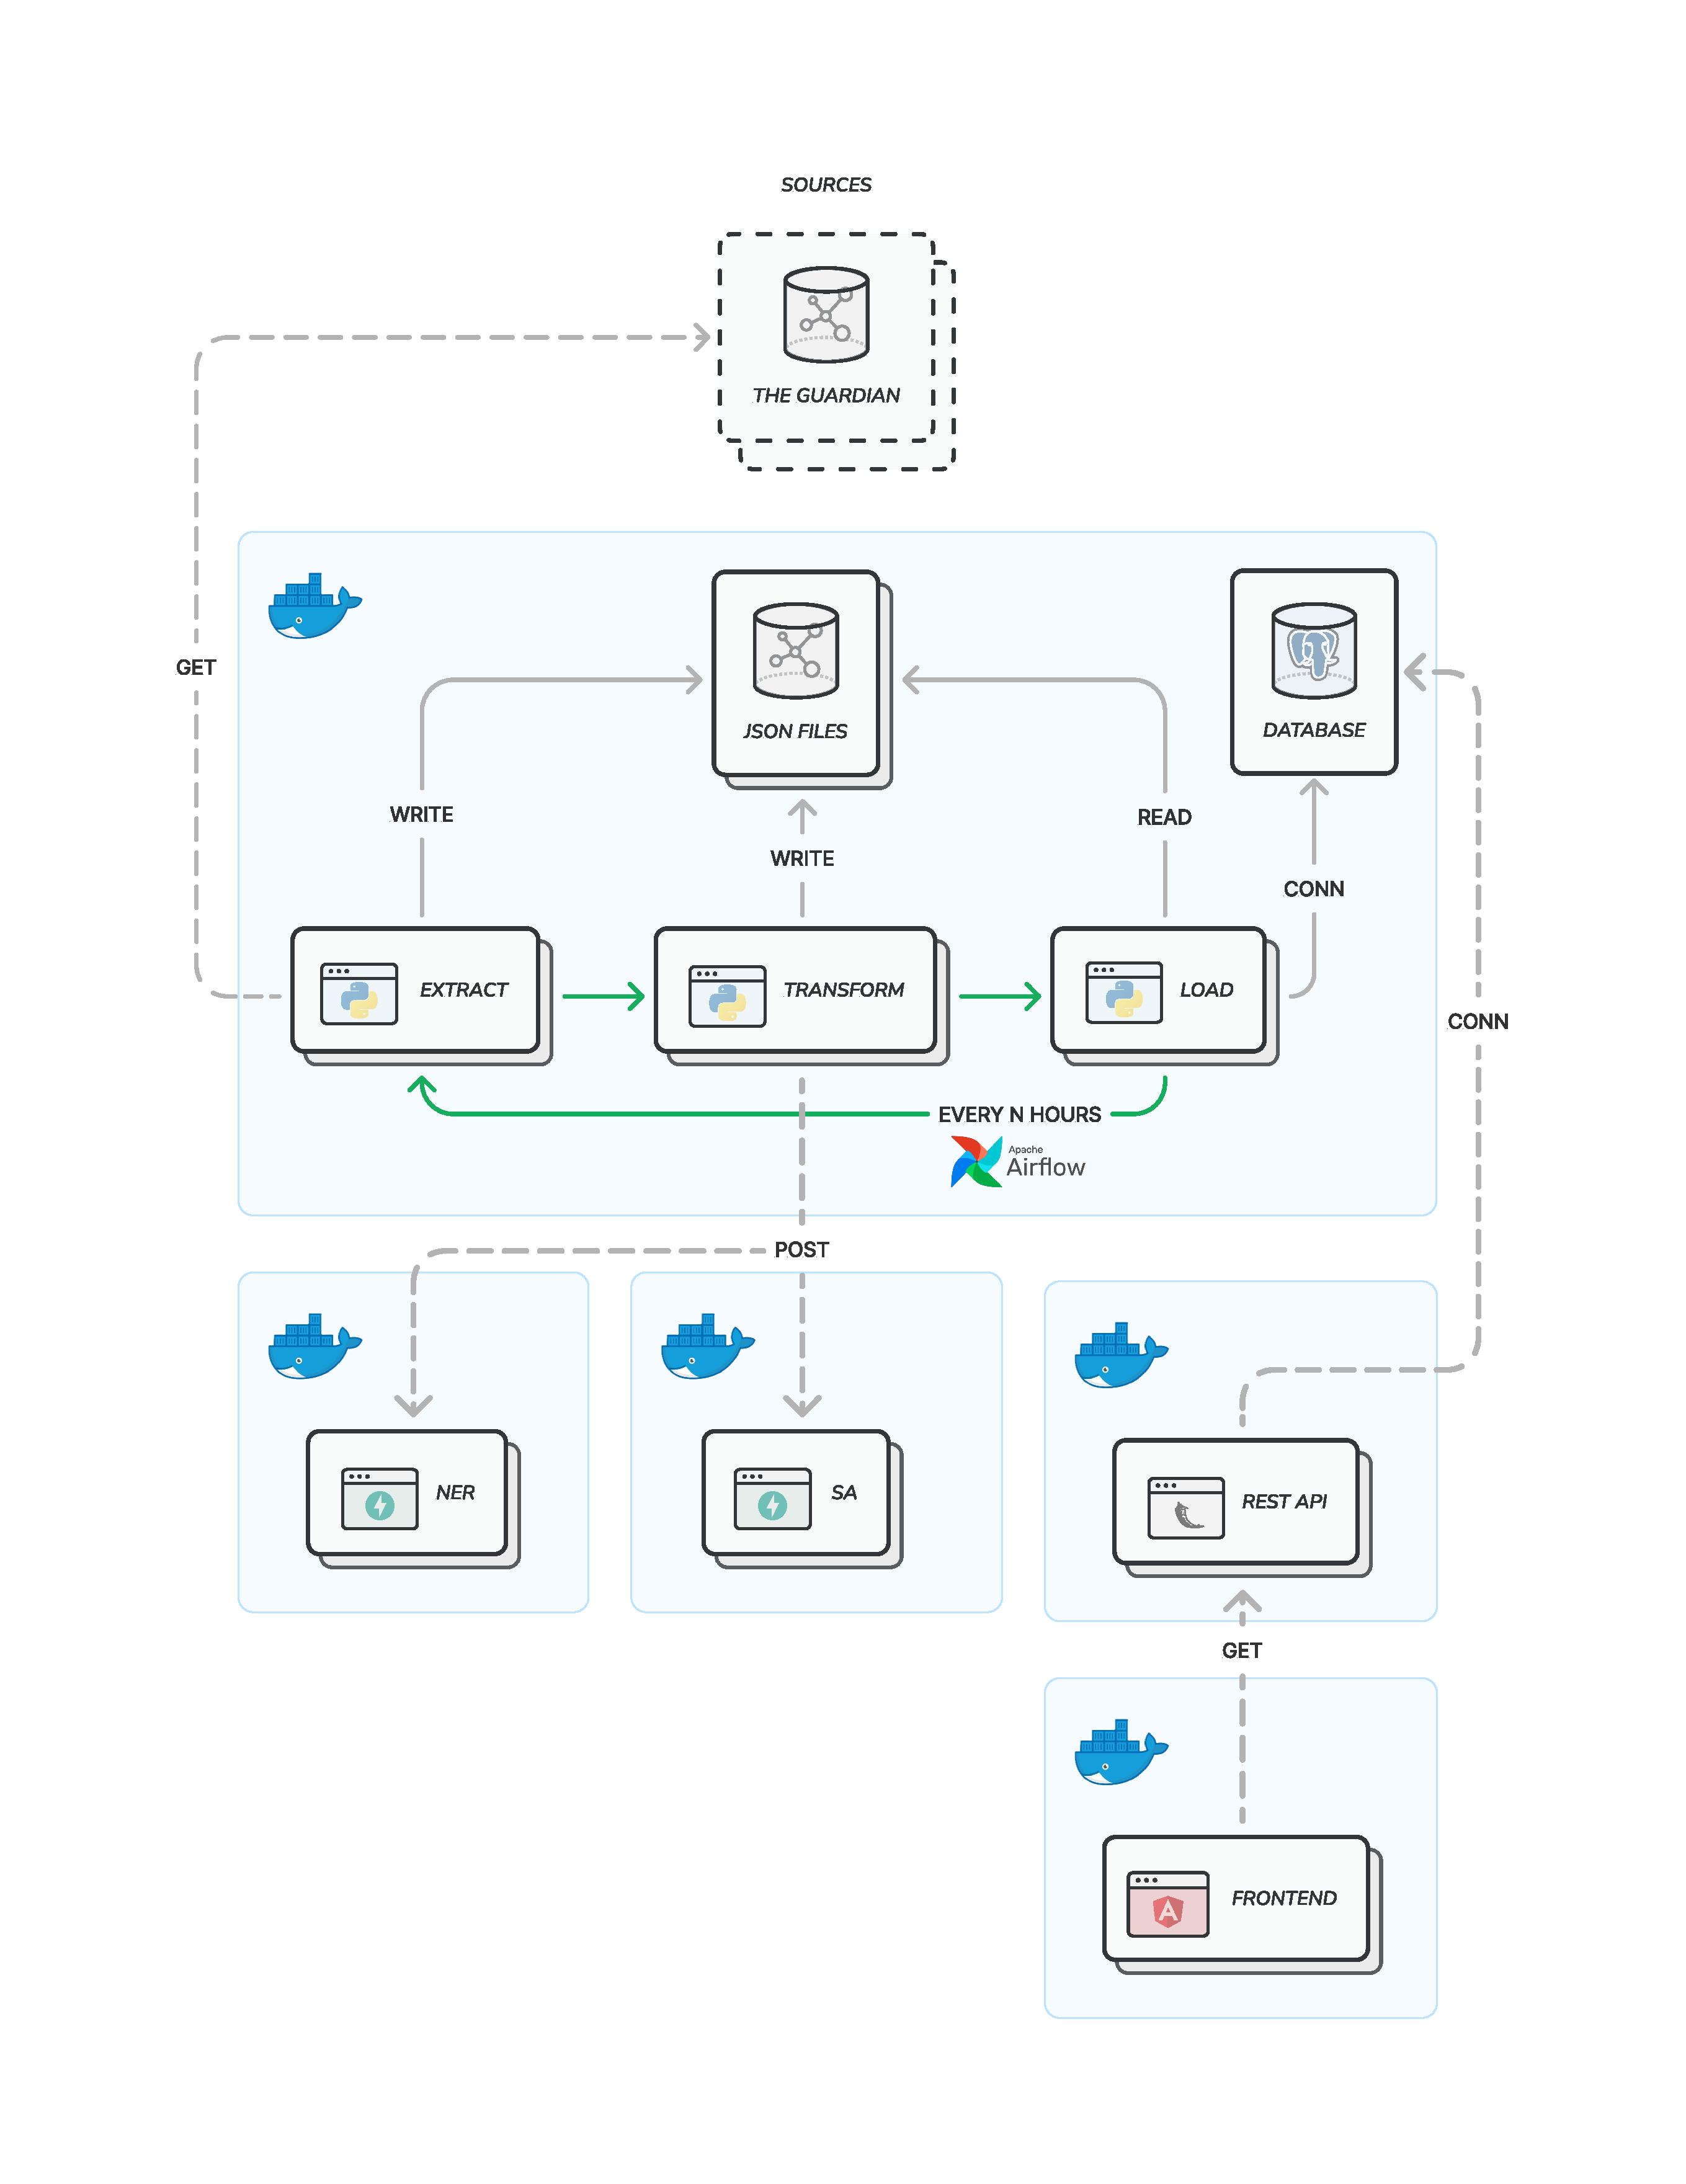
\includegraphics[width=\textwidth]{img/architecture/architecture-high.pdf}
    \caption{The application's high-level architecture containing individual services and their communication. Where N hours is a variable, which will be set to 4 hours in the current version.}
    \label{fig:architecture-high}
\end{figure}

\section{Backend}
\label{sec:architecture-backend}
The backend is divided into several services, each with a distinctly defined role. This section describes each service and the reasons for their division and usage.

\subsection{Extract Transform Load Service}
\label{subsec:architecture-etl}
The \acrshort{etl} service is responsible for acquiring data from external sources, transforming it, and storing it in the database. This process includes three phases:

\begin{itemize}
\item \textbf{Extract:} Acquiring data from the Guardian through Open Platform and saving it to files for further processing.
\item \textbf{Transform:} Transforming the data, including communication with \acrshort{ner} and SA services to extract entities and analyse sentiment. Results are saved to files.
\item \textbf{Load:} Storing the transformed data from files to the database.
\end{itemize}

To facilitate the \acrshort{etl} process, the application uses the Apache Airflow\footnote{\href{https://www.airflow.apache.org}{https://www.airflow.apache.org}} framework as a task orchestrator. Airflow is an open-source tool for planning and managing the flow of data tasks. This framework was chosen because it can schedule and execute tasks in a specific order and under certain conditions. It provides a web server that allows us to monitor task status, view logs, and display results. The scheduler triggers tasks based on a defined schedule while the executor executes these tasks. The application uses the local executor, which runs tasks in parallel on the same machine.

This service also includes two PostgreSQL, in short Postgres, databases. The first database manages the operation of Airflow, while the second database stores the results of the \acrshort{etl} process. Additionally, Airflow itself recommends using a Postgres database to store metadata. The choice of Postgres for article-related data is based on its reliability and ability to process large amounts of structured data. It provides a robust relational model ideal for data such as articles, companies, and sentiments. This model allows for efficient data storage in well-defined tables with relationships between them using foreign keys, ensuring data integrity and facilitating complex querying.

Since we are covering a scheduling pipeline for processing text data, which repeats at regular intervals, it is necessary to ensure that data is constantly available. Therefore, replication of all data in the database as temporary copies of tables occurs at the beginning of the \acrfull{dag} before the extract phase. The original data is deleted from these tables to free up space for new data that will be processed during the current run of the pipeline. By creating copies, we ensure users always have access to data, even during insertion, preventing disruptions. After the load phase, at the end of the \acrshort{dag}, the temporary tables and their data are removed when all the new data are successfully inserted into the original tables, and subsequent additional tasks are finished.

Considering that the data after the transform phase contains only entities as tickers and their associated sentiments, obtaining additional information about the company based on the ticker is necessary. For this purpose, the application uses the Yahoo Finance Python library, which we have used in previous chapters. This library allows obtaining company data such as the name, industry, and website. These pieces of information are then obtained and stored in the database during the load phase after loading the transformed data. Once the data is loaded into the database, we will have information about all the tickers available and will not need to obtain data repeatedly during the transformation. Finally, unnecessary articles that do not contain an entity are removed. This process ensures that only relevant data is stored in the database, reducing unnecessary data storage and improving data quality, see Figure \ref{fig:architecture-etl-highest}.
%\clearpage
%overflow todo
\begin{figure}[htbp]
    \centering
    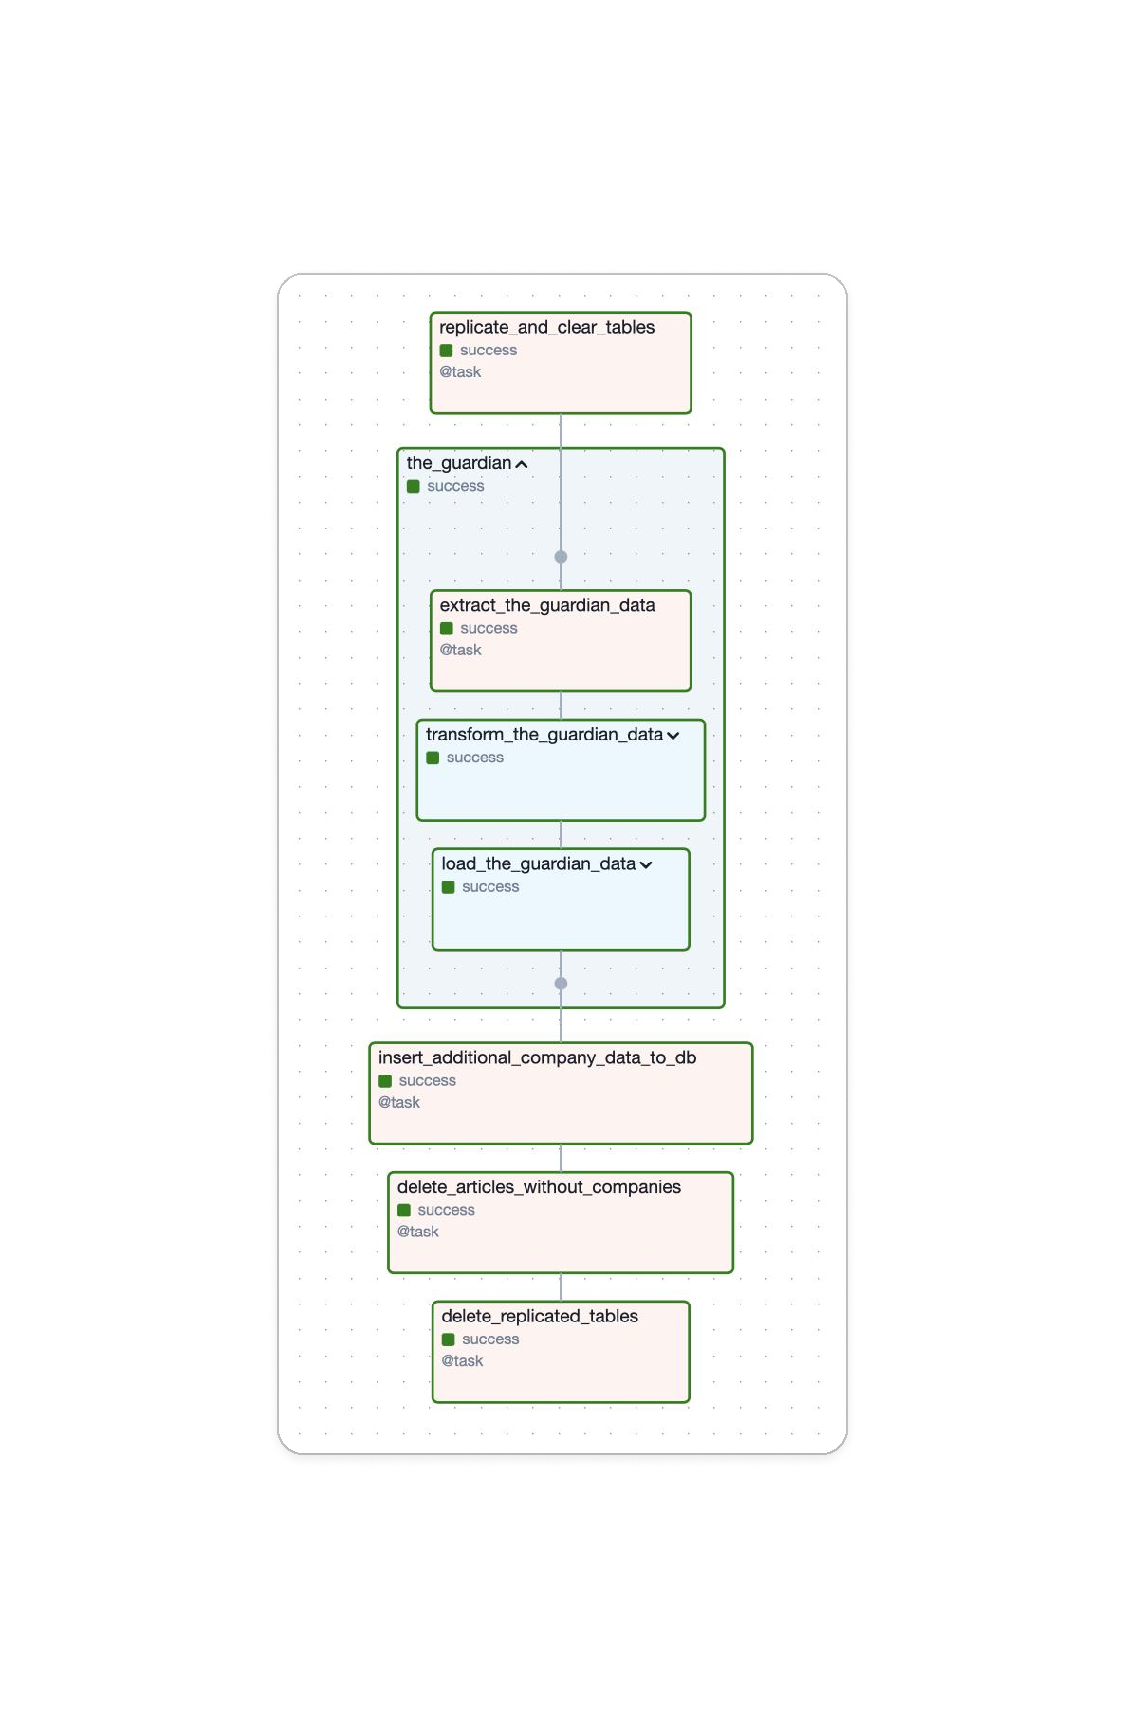
\includegraphics[width=0.6\textwidth]{img/architecture/etl-highest.pdf}
    \caption{The \acrshort{dag} of Guardian's \acrshort{etl} phases, including four additional tasks for data tables replication and cleaning, insertion of additional company data, deletion of articles without companies, and deletion of replicated tables. Oriented from top to bottom.}
    \label{fig:architecture-etl-highest}
\end{figure}

\subsubsection{Database Details}
\label{subsubsec:architecture-etl-database-details}
As mentioned, Postgres is the primary database for storing data and utilises the relational model. Our database implementation has several tables, as shown in Figure \ref{fig:architecture-etl-database-schema}. In addition, the Database Markup Language\footnote{\href{https://dbml.dbdiagram.io/home}{https://dbml.dbdiagram.io/home}} (DBML) schema can also be found in the attatchment\footnote{Located in the directory directory /docs/database/}.

\begin{figure}[htbp]
    \centering
    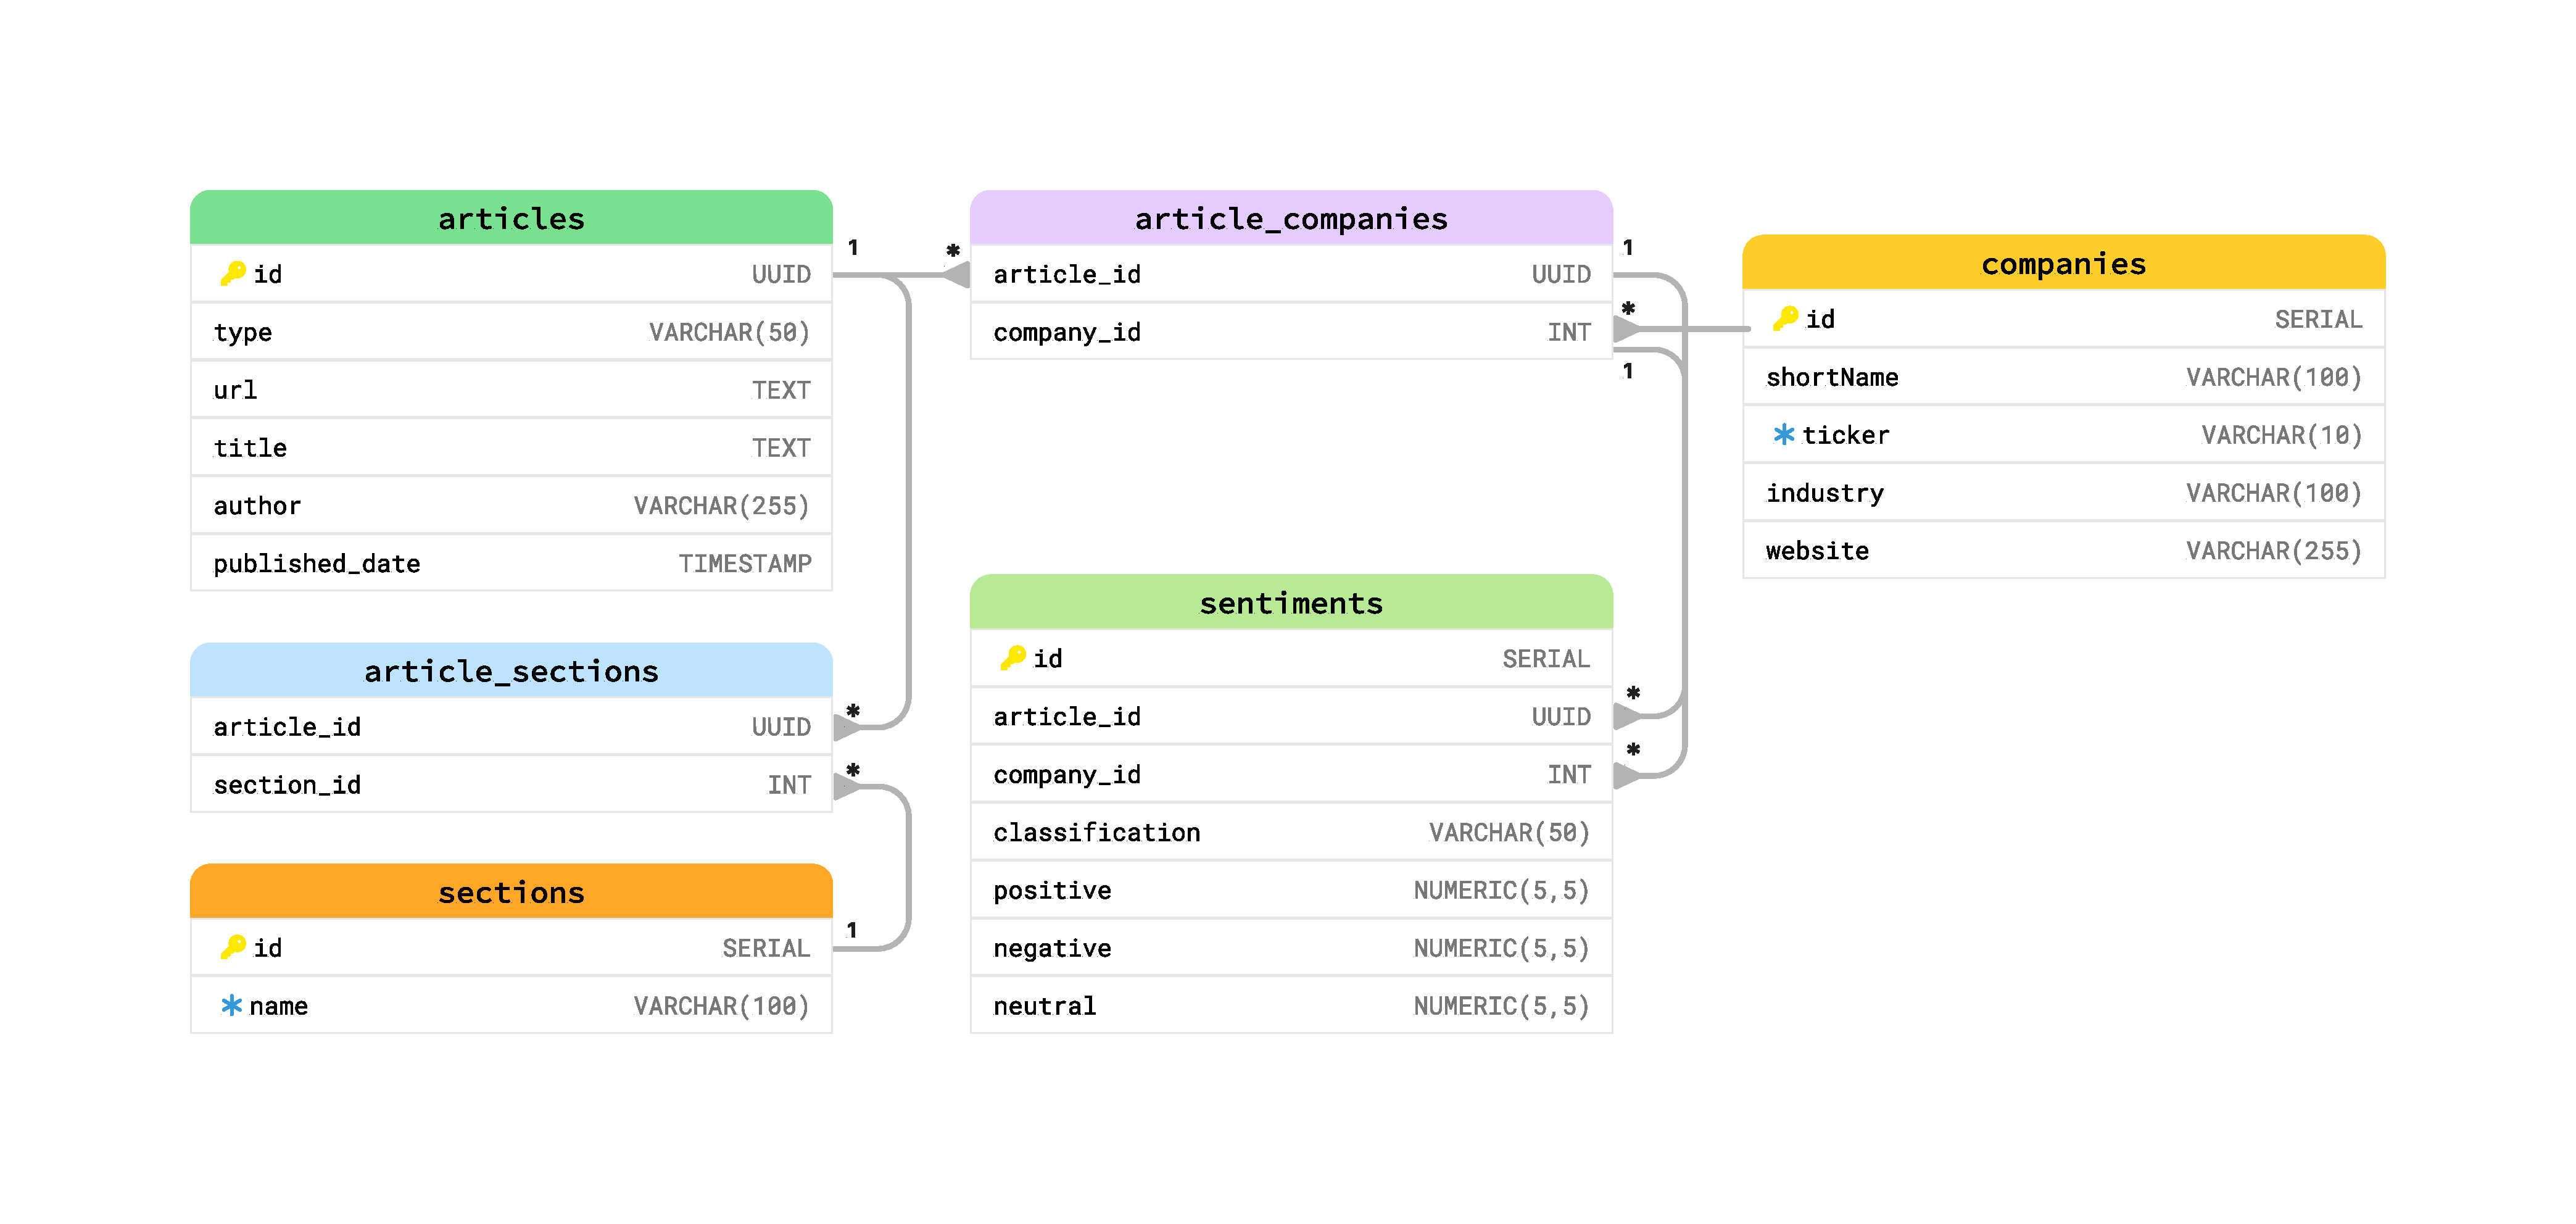
\includegraphics[width=\textwidth]{img/architecture/database-schema.pdf}
    \caption{Relational schema of \acrshort{etl} service database for storing article-related data.}
    \label{fig:architecture-etl-database-schema}
\end{figure}

Given the extensive utilisation of the join operation in our queries, we have established the three supplementary indexes on columns commonly employed for table joins. The following indexes are designed to improve the performance of queries that join data from these tables and respond to frequent queries more efficiently:

\begin{itemize}
    \item \textbf{\textit{idx\textunderscore article\textunderscore companies\textunderscore article\textunderscore id\textunderscore company\textunderscore id}} for columns \textit{article\textunderscore id} and \textit{company\textunderscore id} on the \textit{article\textunderscore companies} table
    \item \textbf{\textit{idx\textunderscore sentiments\textunderscore article\textunderscore id\textunderscore company\textunderscore id}} on the sentiments table for columns \textit{article\textunderscore id} and \textit{company\textunderscore id}
    \item \textbf{\textit{idx\textunderscore article\textunderscore sections\textunderscore article\textunderscore id\textunderscore section\textunderscore id}} on the \textit{article\_ }\textit{sections} table for columns \textit{article\textunderscore id} and \textit{section\textunderscore id}
\end{itemize}

Suppose we would like to incorporate more types of entities into the database in the future, such as people, events, or products with various relationships between them. In that case, we might consider using a graph database like Neo4j. Nevertheless, the relational model in the current stage of the application version is the most suitable choice for storing current type of data.

\subsubsection{Extract Details}
\label{subsubsec:architecture-etl-extract-details}
During implementation, we focused on making connecting additional sources for extraction effortless. Currently, we use only one source, the Guardian, for reasons outlined in Chapter \ref{chap:textual-data}. If we wanted to add more sources, it would be cautious to discuss and consider a filter to determine how similar articles from different sources are to avoid duplicating sentiment values from articles with the same content. Alternatively, we could account for this information in another way, such as weighting the sentiment based on the source's popularity and potential reach, which could impact the market.

Each source creates a separate tasks pipeline in Airflow within a single \acrshort{dag}, containing all phases of the \acrshort{etl} process. This approach allows us to easily add new sources without modifying the existing pipeline. The phases are divided into tasks and task groups, ensuring clarity, comfortable navigation in the code, simple implementation, and the possibility of parallel execution of individual tasks.

Specifically, extraction is performed as a single task for the Guardian source by requesting the Open Platform. The time frame for extracting articles is set to three months. During this period, about $1000$ articles is extracted, focusing on the business and technology sections. The endpoint paginates data in batches of $200$ articles. After determining the number of pages, a task is created for each page to retrieve the data and save it to a file. This method was chosen because the API limits the number of articles we can retrieve simultaneously, making pagination necessary. On the other hand, we can use this guideline to clearly define the data size distribution for individual tasks. Thus, it allows us to monitor the extraction process and ensure parallel execution in the subsequent transform phase.

\subsubsection{Transform Details}
\label{subsubsec:architecture-etl-transform-details}
The transform phase begins by reading the extracted data stored in files. It simplifies storing the final transformed data without copying and updating existing files. This ensures the data is available even if an error occurs in the subsequent phases and allows for continuous monitoring. Airflow provides cross-communication (X-Coms) data, which is loaded into metadata and can be easily passed between tasks. Although we know about the limitations, it is generally not recommended to transfer extensive data (approximately $1$ GB) using X-Com with a Postgres database supporting Airflow \parencite{laura2023-medium}. In our case, individual files of $200$ articles with file sizes ranging from $1$ to $2$ MB, making it acceptable with a substantial reserve.

The \acrshort{ner} task pulls article content data from X-Coms and sends the content to the \acrshort{ner} service \acrshort{api} endpoint. The response contains entities, each with its ticker and the substring defining the entity in the text. The result is then pushed into X-Coms as separate data. It ensures that the \acrshort{ner} task results are available for the subsequent \acrshort{sa} task.

The \acrshort{sa} task pulls article content and entity data from X-Coms. It sends the content and identified entities to the \acrshort{sa} service API endpoint, which responds with sentiments for each entity. The results are then pushed into X-Coms as another data collection containing entities and their sentiments for each article.

The results from X-Coms are combined with the original article data from the extract phase, excluding the content that no longer needs to be stored. The combined results are saved into files used in the subsequent load phase. This approach ensures a transparent and efficient processing workflow, which can be defined in task groups containing individual task dependencies, allowing for parallel data processing (see Figure \ref{fig:architecture-etl-transform}).

\begin{figure}[htbp]
    \centering
    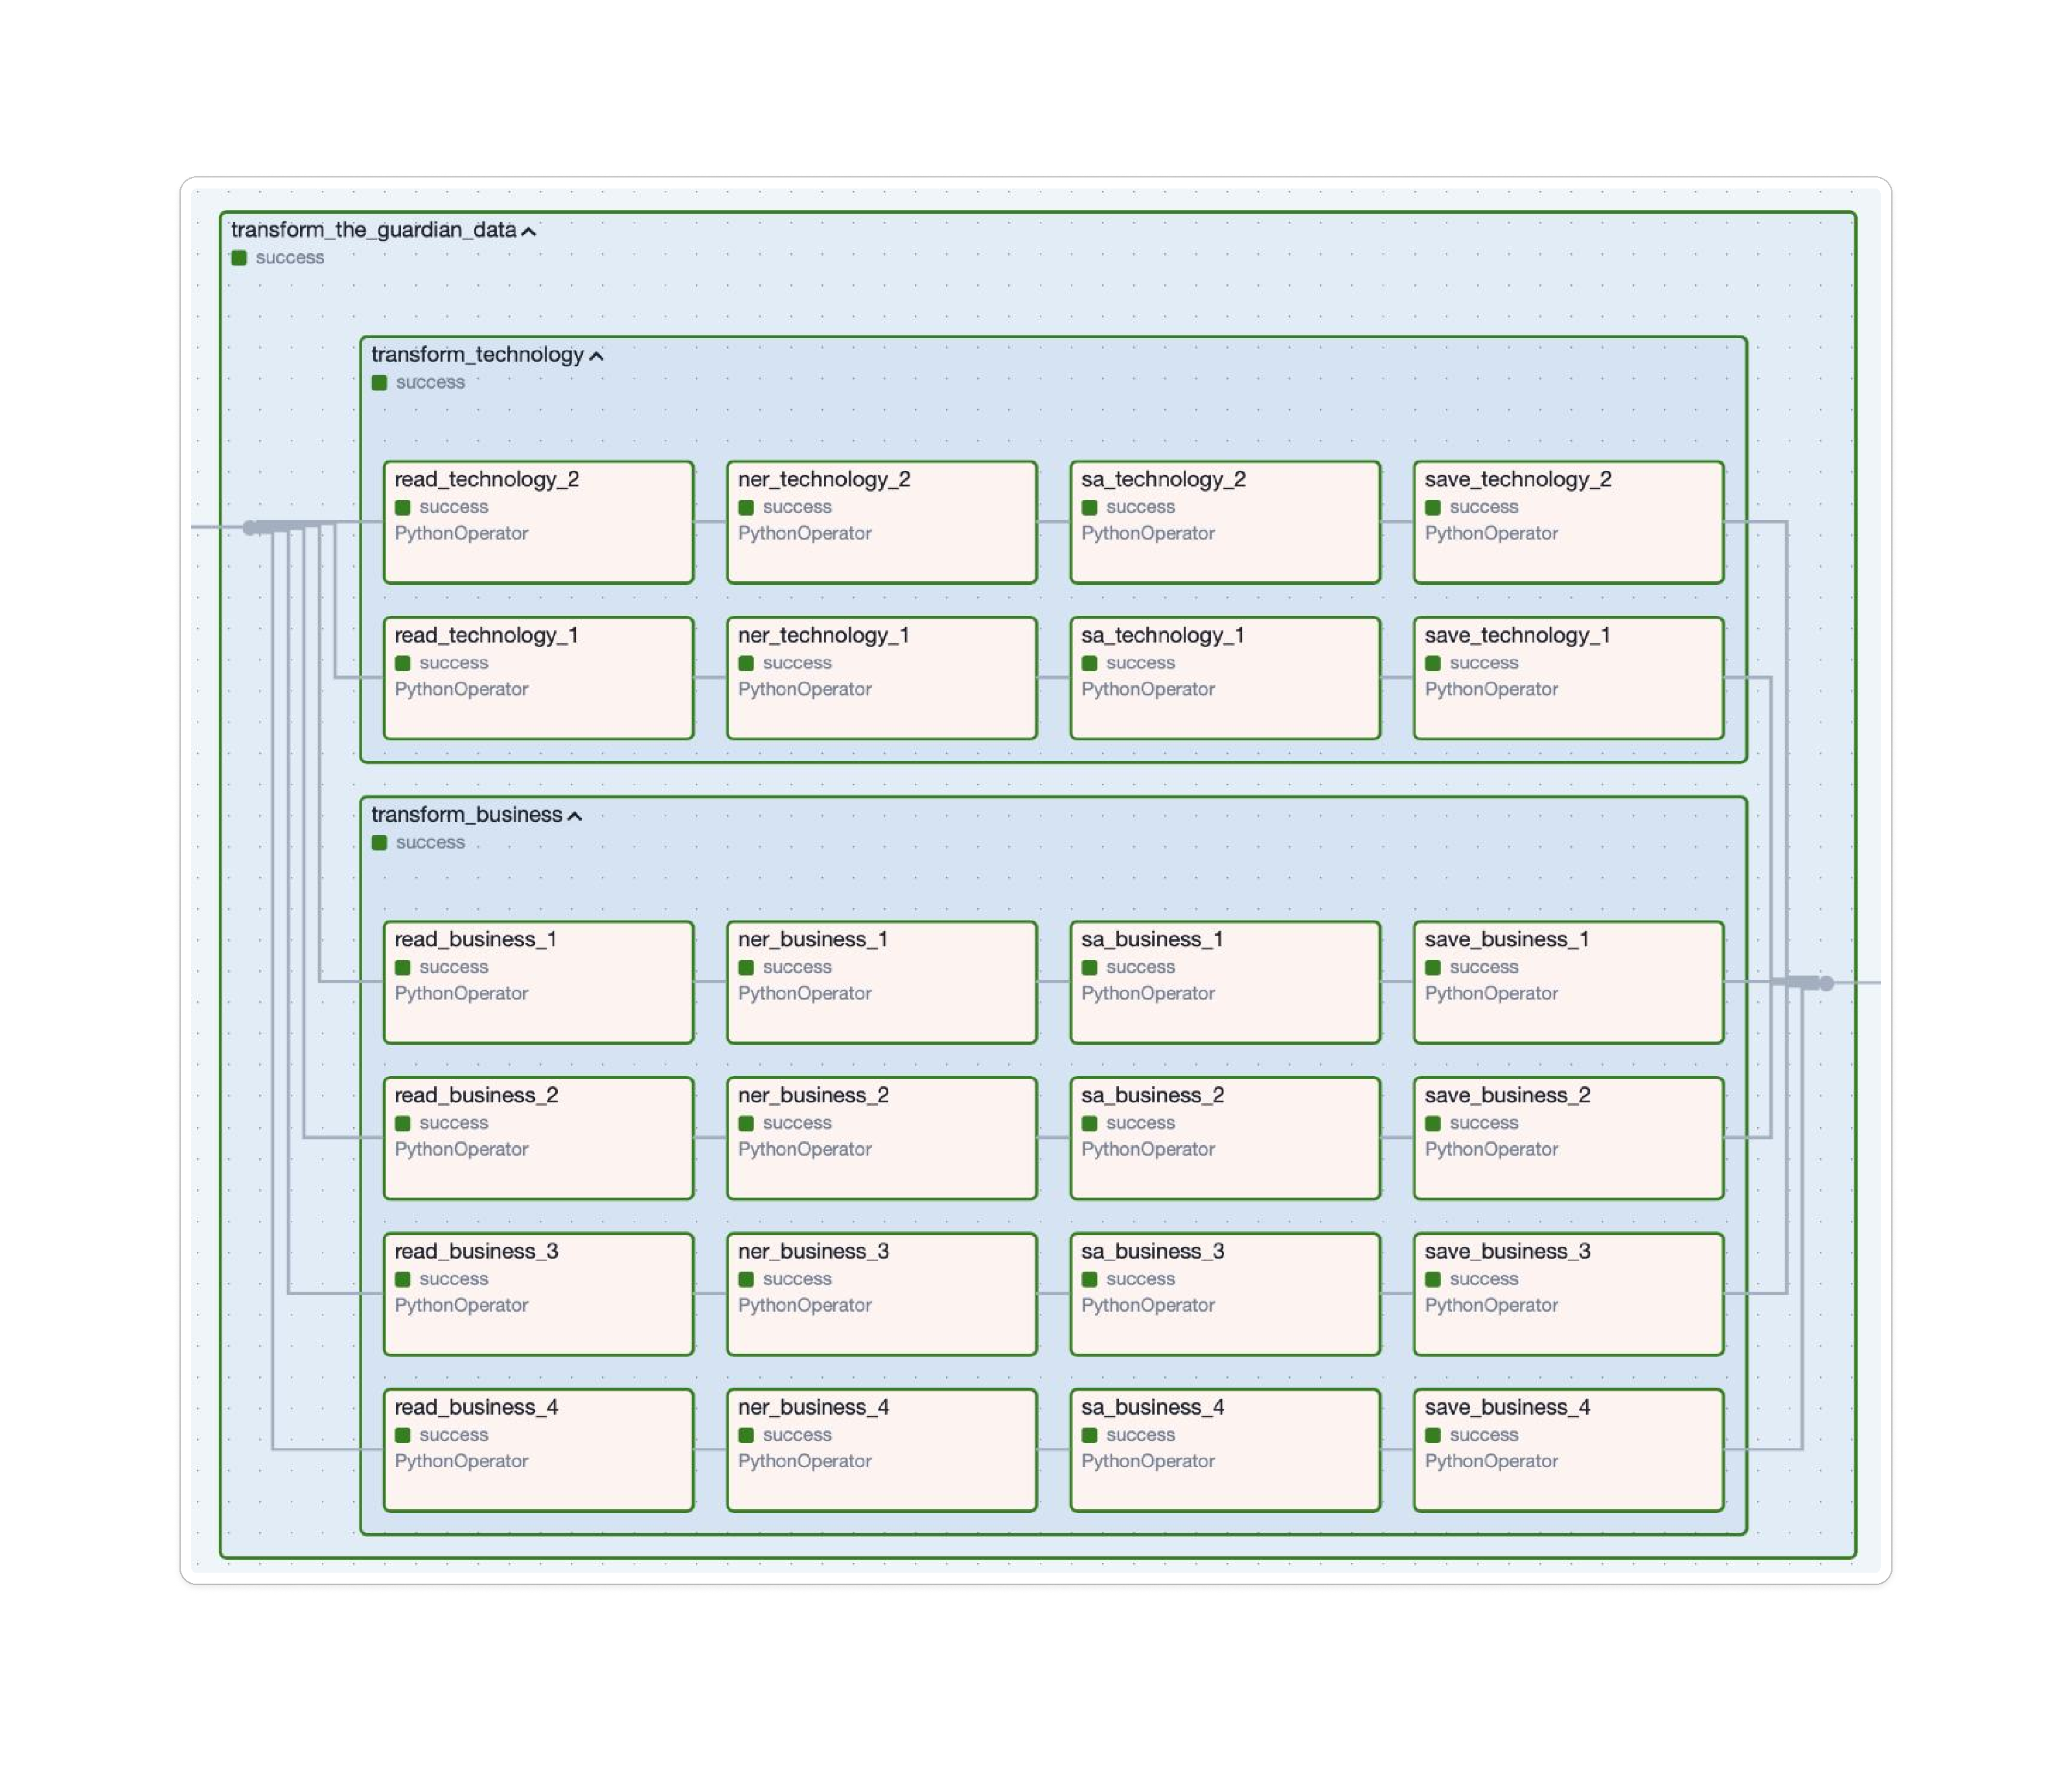
\includegraphics[width=\textwidth]{img/architecture/etl-transform.pdf}
    \caption{The transform phase task groups and its tasks in the \acrshort{dag} of Guardian's \acrshort{etl} process. Directed from left to right.}
    \label{fig:architecture-etl-transform}
\end{figure}

\subsubsection{Load Details}
\label{subsubsec:architecture-etl-load-details}
The load phase begins with sequentially transformed data bulk loading into the database. In the current version, we do not employ loading in parallel because we have found that the approximate load duration time (see Table \ref{fig:architecture-etl-load}), in addition to a slowdown due to extra indexes, is acceptable, and parallel loading is unnecessary. It could lead to collisions where multiple sources simultaneously write to the same table. This approach could compromise data integrity and lead to database errors, especially when articles containing the same entities are inserted into the table concurrently. While row locking could mitigate this issue, it would slow down the entire process and increase system complexity, which could be counterproductive given the current data volume. Therefore, we prefer sequential data loading from a single source. The entire process of the Load phase is illustrated in Figure \ref{fig:architecture-etl-load}.

After loading data from individual task groups of sections, there is a task to insert additional company data into the database. This task involves inserting previously mentioned data such as short name, industry, and website from Yahoo Finance. Subsequently, there is a task that removes articles that do not contain any tickers. These articles are unusable to us, and their removal helps maintain data cleanliness in the database and reduces unnecessary database load.

\begin{table}[ht]
    \centering
    \caption{The approximate duration of individual tasks and task groups in the \acrshort{etl} process for the Guardian source.}
    \label{table:etl-task-durations}
    \begin{tabular}{l c}
        \hline
        \textbf{Task \& Task Group} & \textbf{Duration [min]} \\
        \hline
        replicated\_and\_clear\_tables & 0.02 \\
        insert\_additional\_data & 0.98 \\
        delete\_articles\_without\_companie & 0.02 \\
        delete\_replicated\_tables & 0.02 \\
        \hline
        \textbf{extract\_the\_guardian\_data} & 0.09 \\
        \hline
        \textbf{transform\_the\_guardian\_data} & 44 \\
        \hline
        transform\_business & 42 \\
        transform\_technology & 44 \\
        \hline
        \textbf{load\_the\_guardian\_data} & 0.35 \\
        \hline
        load\_technology & 0.08 \\
        load\_business & 0.22 \\
        \hline
    \end{tabular}
\end{table}

\begin{figure}[ht]
    \centering
    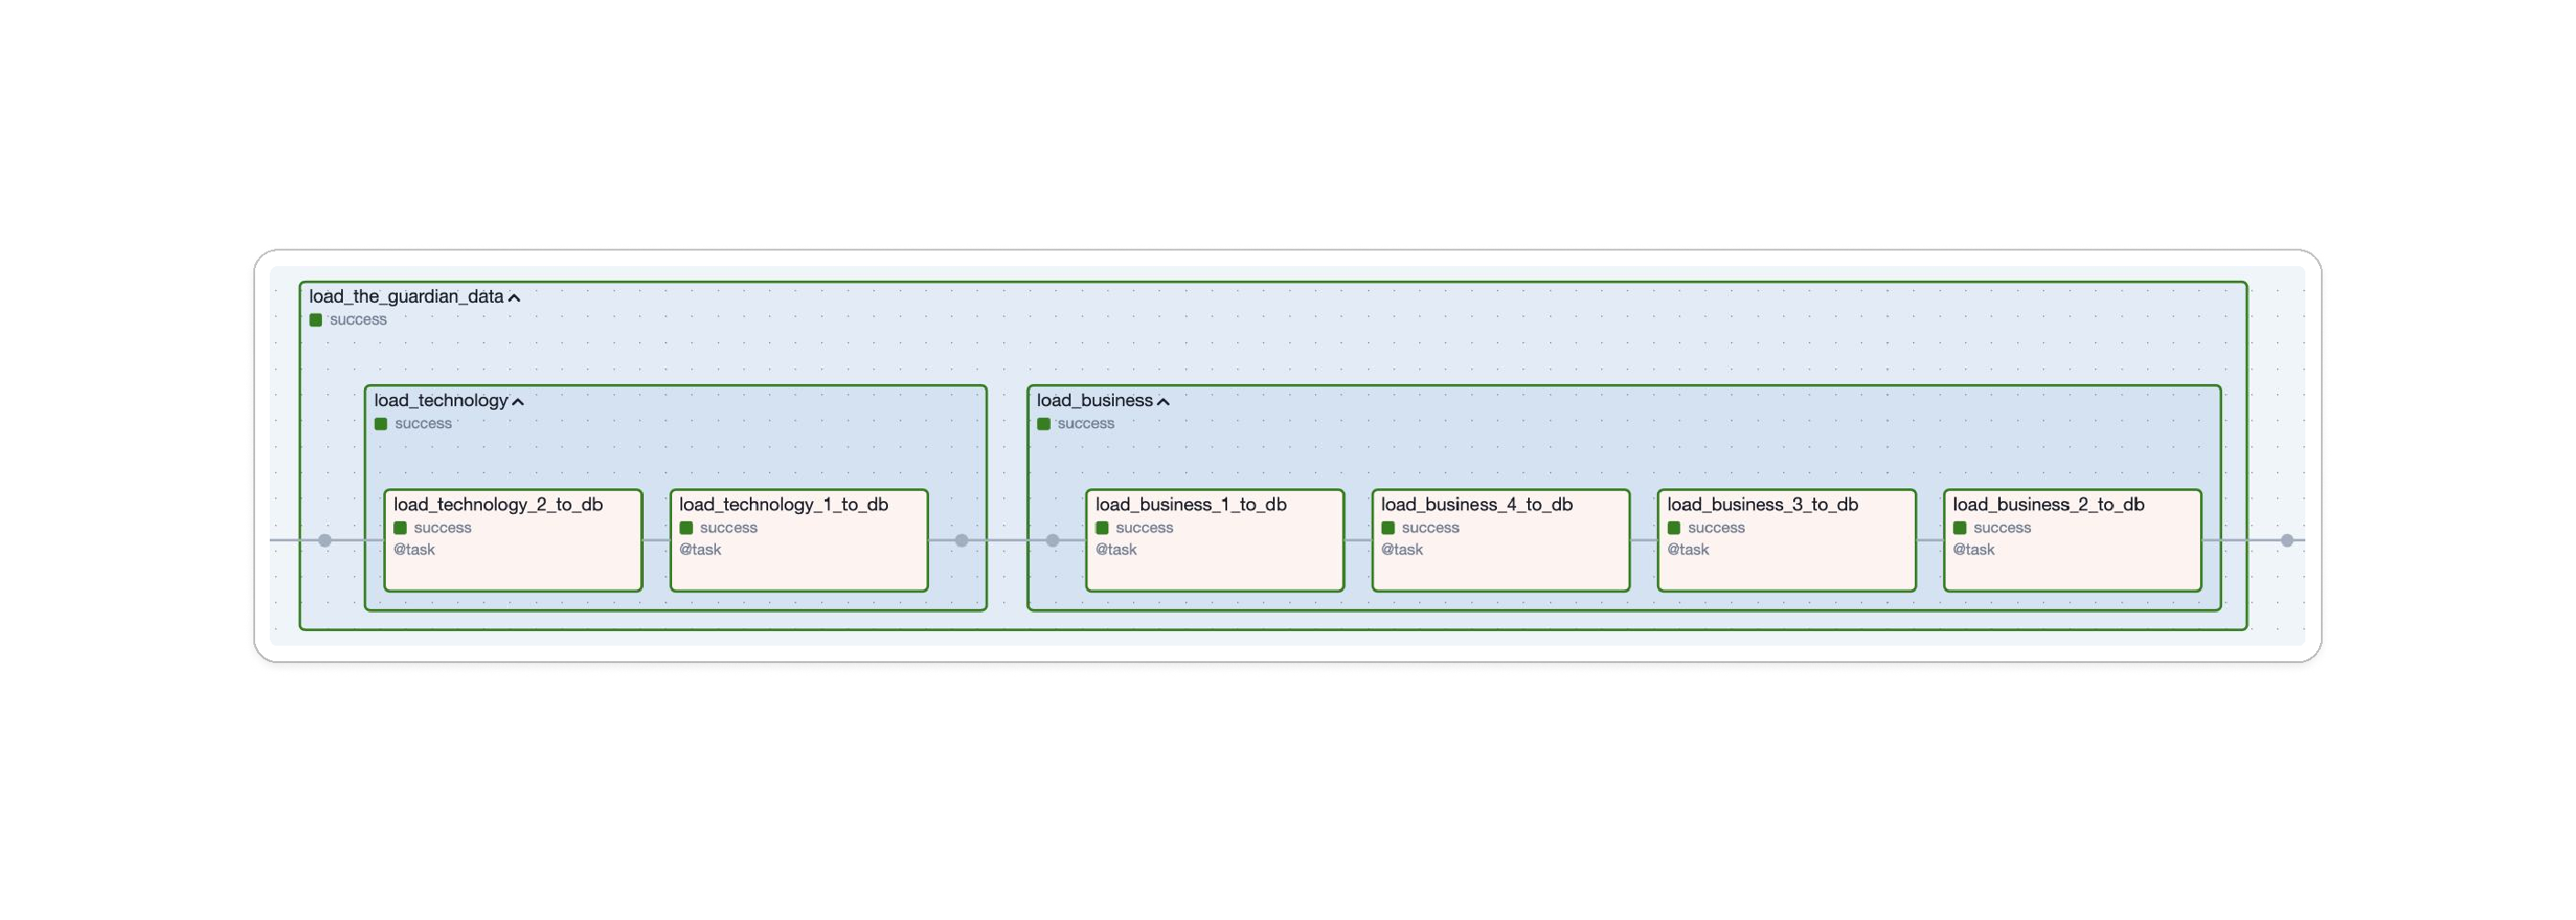
\includegraphics[width=\textwidth]{img/architecture/etl-load.pdf}
    \caption{The load phase task groups and its tasks in the \acrshort{dag} of Guardian's \acrshort{etl} process. Directed from left to right.}
    \label{fig:architecture-etl-load}
\end{figure}

According to Tabel \ref{table:etl-task-durations}, the transformation of the technology section, even though it contains only two pages (files) of articles, is completed in a similar time as the business section, which is twice as extensive. This is due to the distribution of jobs among workers, of which we have $16$ in our setup. The entire \acrshort{dag} work is automatically divided among the workers. However, the transformation results primarily depend on the response times of the \acrshort{ner} and \acrshort{sa} services. The \acrshort{sa} service, in particular, slows down the process owing to the computationally intensive FinABSA-Longer model, which has limited speed due to article content length. The average duration of \acrshort{ner} task groups is approximately $4$ minutes, while the average duration of \acrshort{sa} task groups\footnote{\acrshort{ner} task group in one task instance processes all 200 articles, whereas \acrshort{sa} processes only those that contain a ticker after NER is finished.} is $33$. The total runtime for a single execution of the entire pipeline, from extraction to loading and removing temporary tables, is approximately $45$ minutes. In the following subsection, we will examine the construction of requested services. Lastly, we propose how the \acrshort{dag} distribution might look by adding two more sources, shown in Figure \ref{fig:architecture-etl-sources}.

\begin{figure}[ht]
    \centering
    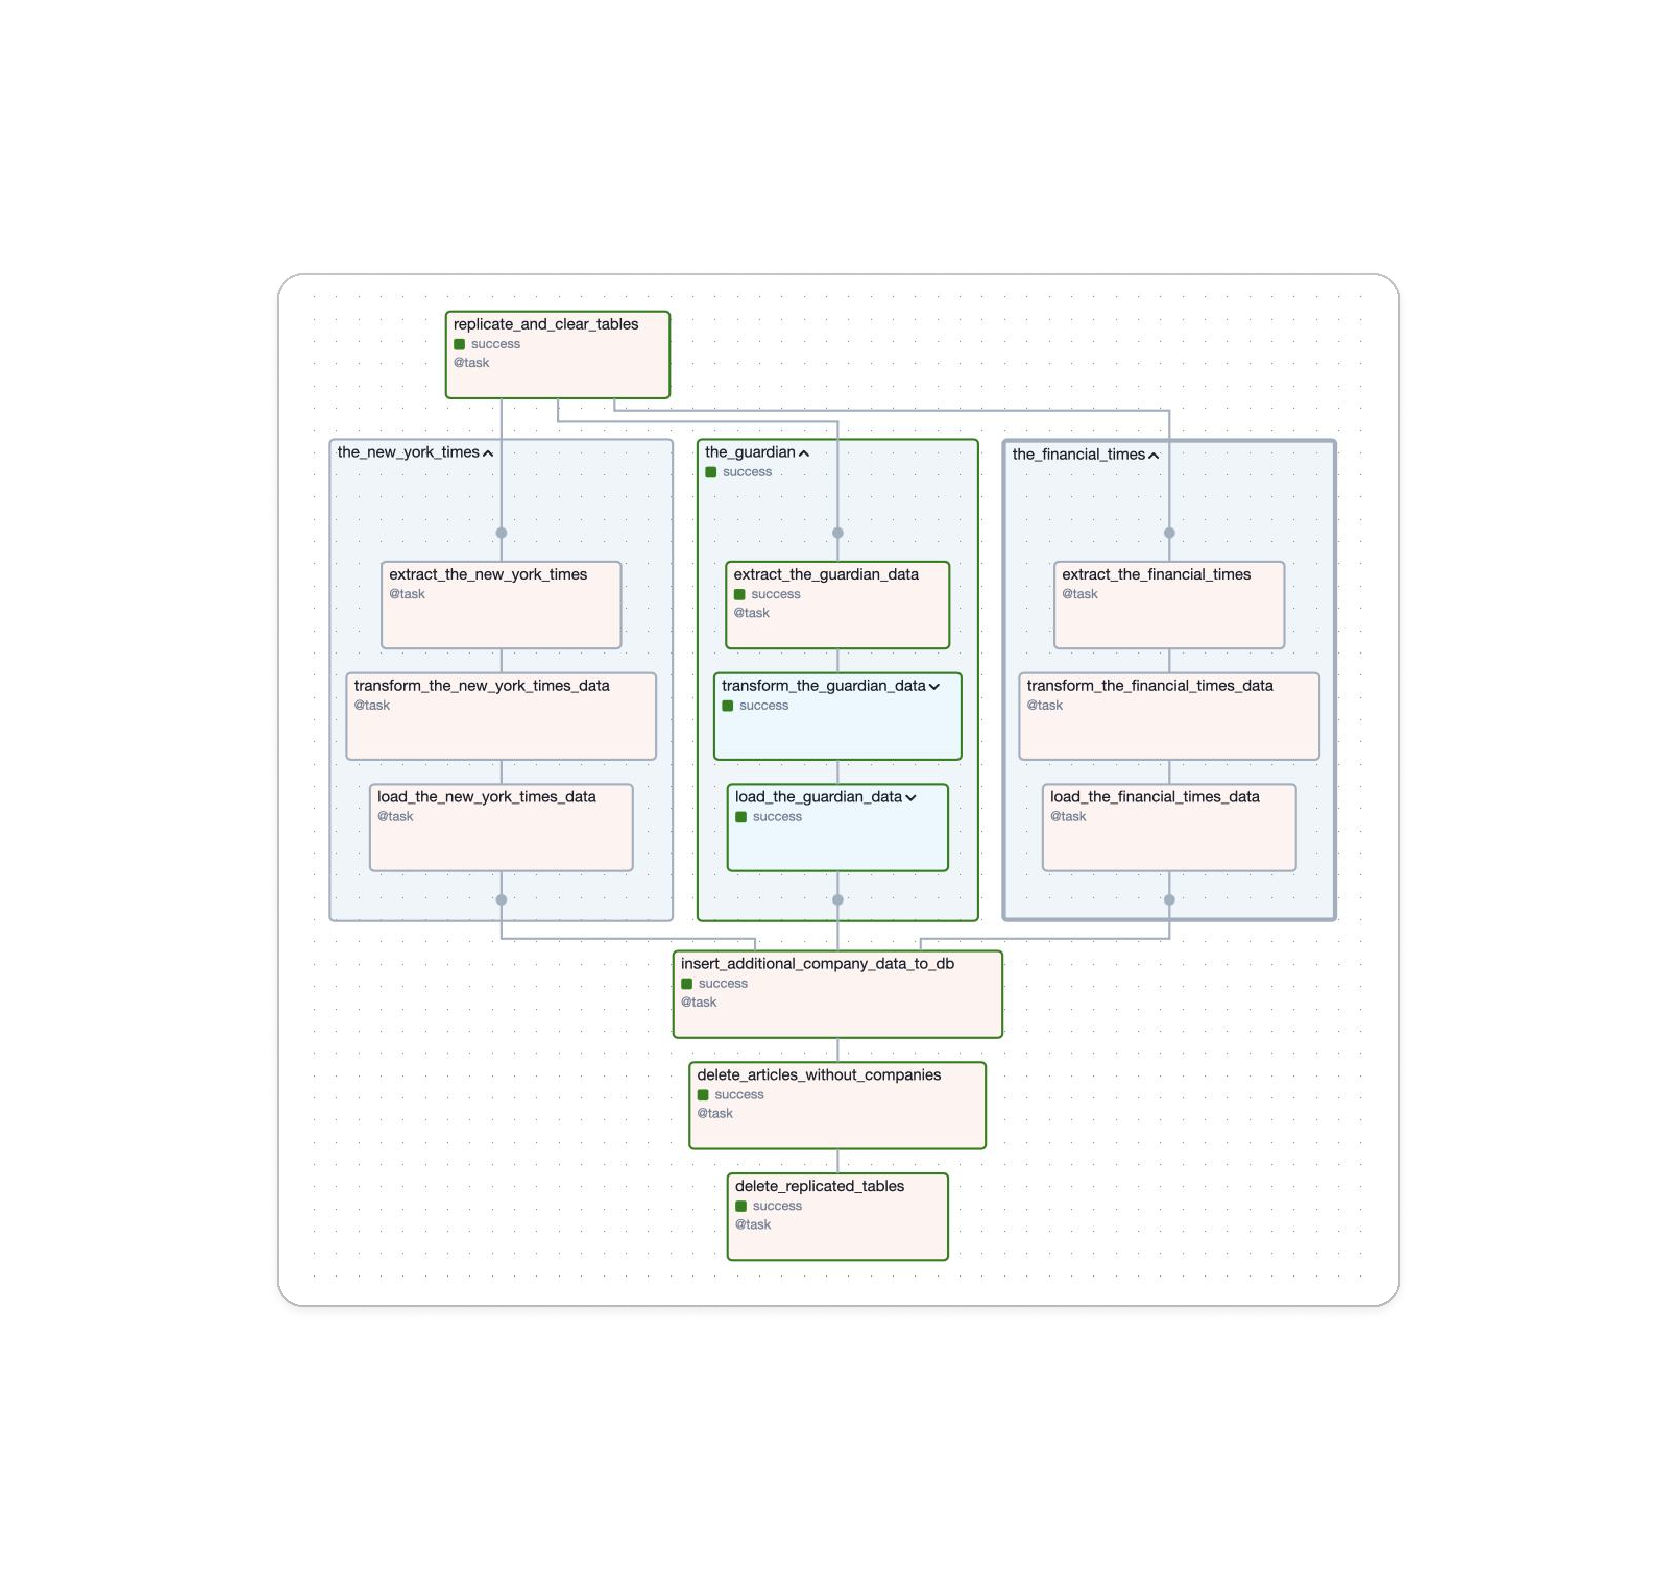
\includegraphics[width=0.8\textwidth]{img/architecture/etl-sources.pdf}
    \caption{The \acrshort{dag} of \acrshort{etl} phases for multiple sources, including the Guardian, New York Times, and Financial Times.}
    \label{fig:architecture-etl-sources}
\end{figure}

As mentioned, the time frame for extracting articles is set to three months. During this period, the database in the technology and business sections typically contains approximately the number of records indicated in Table \ref{table:architecture-etl-database-records}.

\begin{table}[ht]
    \centering
    \caption{The approximate number of records in the database tables after three months of time frame extraction employs the Guardian as the source focusing on business and technology sections.}
    \label{table:architecture-etl-database-records}
    \begin{tabular}{l c}
        \hline
        \textbf{Table} & \textbf{Records} \\
        \hline
        \textit{articles}       & 543 \\ 
        \textit{companies}      & 180 \\ 
        \textit{sections}       & 2 \\
        \textit{sentiments}     & 1,327 \\
        \textit{article\textunderscore companies} & 1,327 \\
        \textit{article\textunderscore sections}  & 543 \\
        \hline
    \end{tabular}
\end{table}

\subsection{Named Entity Recognition Service}
\label{subsec:architecture-ner}
The \acrshort{ner} service categorises entities in article content data. Its core component is the named entity recognition algorithm, detailed in Chapter \ref{chap:comapny-to-symbol-linking}. We emphasise identifying organisation-type entities and filtering to determine companies\footnote{Reminder that organisations can be considered potential companies. An organisation is defined as a company if it has a ticker.} specifically within the algorithm. This service plays a crucial role in subsequent data processing, as the entities obtained serve as input for the \acrshort{sa} service.

This service operates as a FastAPI\footnote{\href{https://www.fastapi.tiangolo.com}{https://www.fastapi.tiangolo.com}} server, offering a POST request endpoint to extract entities from article content. The output includes a list of entities containing a ticker symbol and a substring representing the entity in the text. Especialy, \acrshort{sa} service then processes substring further in analysis. Upon requesting this endpoint, results are returned to the \acrshort{etl} process during its transformation phase before continuing to the \acrshort{sa} service. The following Figure \ref{fig:architecture-ner-req-res} shows the schema of a POST request to the \acrshort{ner} service for extracting entities from article content and its response.

\begin{figure}[ht]
    \centering
    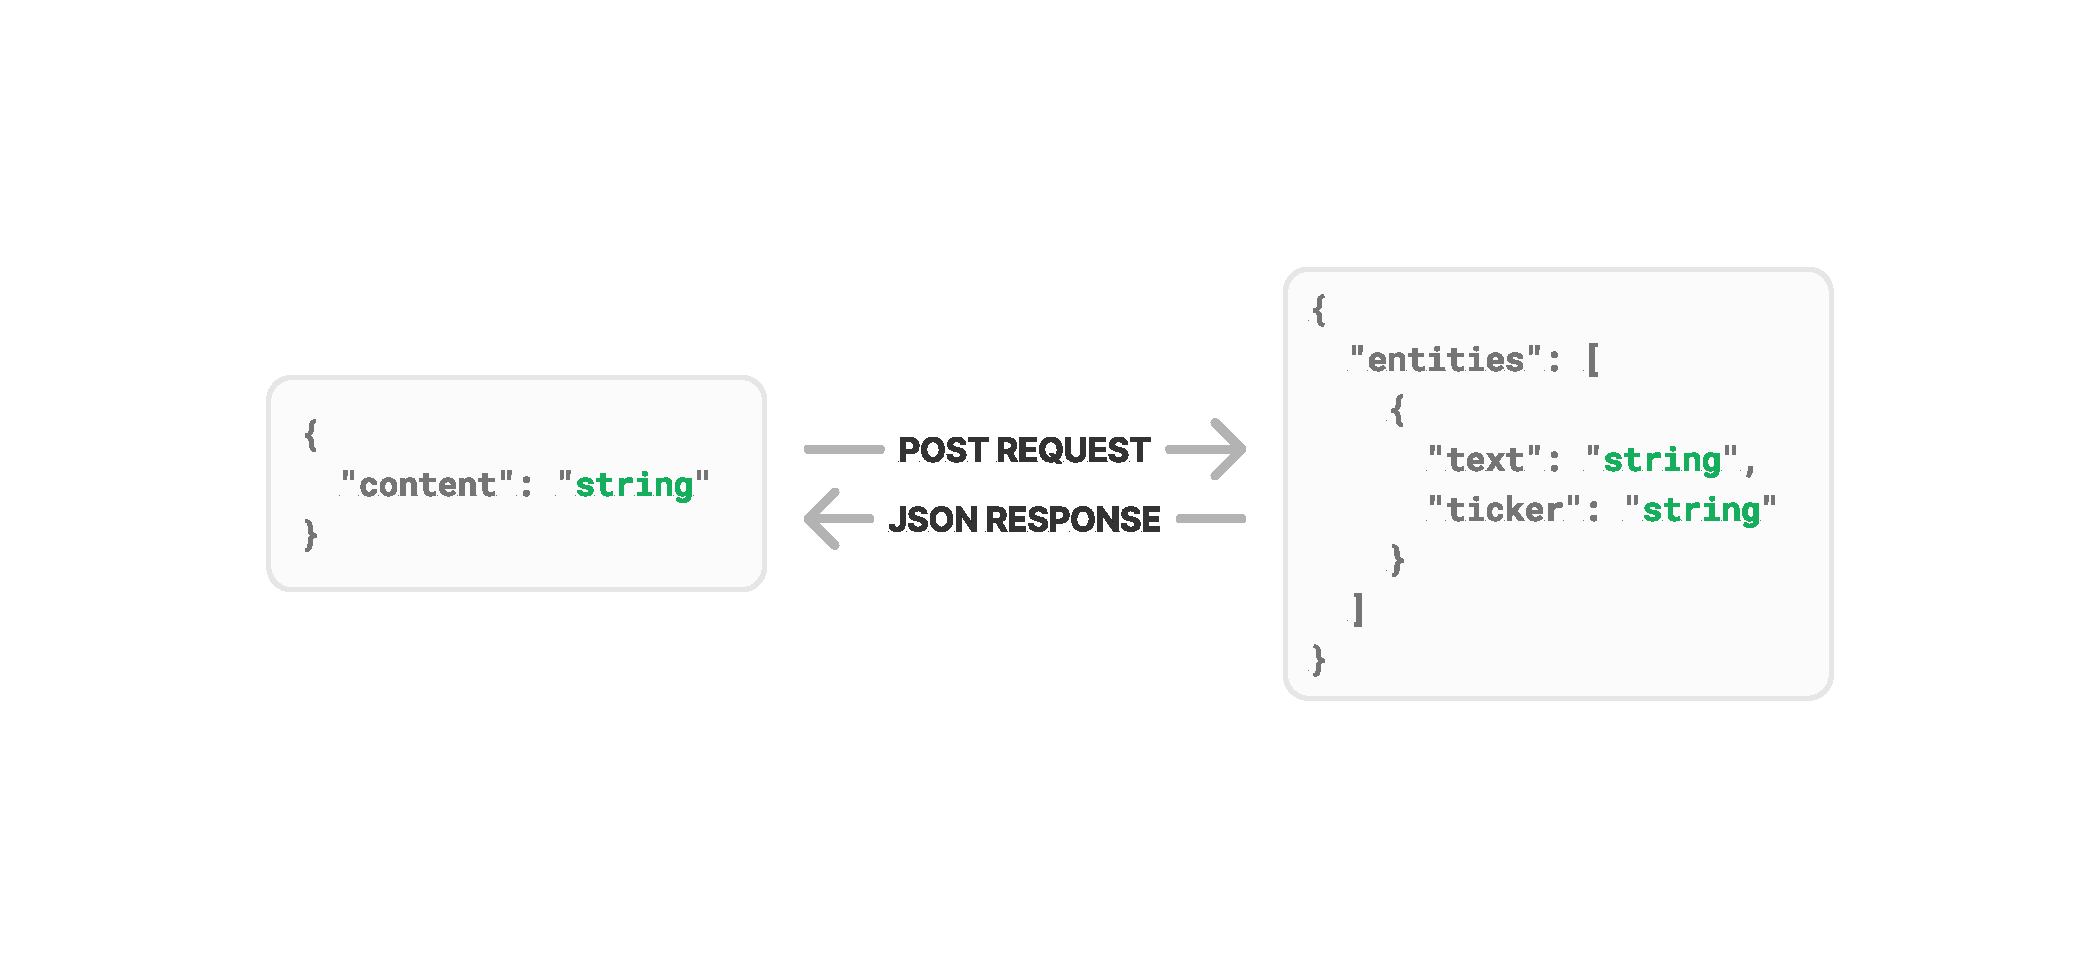
\includegraphics[width=\textwidth]{img/architecture/ner-req-res.pdf}
    \caption{Schema of a POST request to the \acrshort{ner} service for extracting entities from article content and its response.}
    \label{fig:architecture-ner-req-res}
\end{figure}

The need for the fastest response times and efficient data handling drove the choice of the FastAPI framework. Its speed, user-friendly nature, and broad user community are the main reasons for its selection. It integrates seamlessly with the Pydantic library\footnote{\href{https://docs.pydantic.dev/}{https://docs.pydantic.dev/}}, allowing data to be defined as Python classes that automatically generate JSON schemas for data validation within the FastAPI framework. Moreover, FastAPI is built on the Asynchronous Server Gateway Interface\footnote{\href{https://asgi.readthedocs.io/en/}{https://asgi.readthedocs.io/en/}} (ASGI) framework, which is suitable for our querying of Wikidata. The asynchronous implementation of the code allows operations to run independently of the server's main thread, enabling the server to handle more requests and perform other tasks while waiting for a response or processing data retrieved from Wikidata. This is highly desirable for our \acrshort{etl} pipeline, where processing large amounts of data is necessary while maintaining processing speed. Due to the server's limitations on which the \acrshort{ner} service runs, the endpoint is handled by two workers for request processing.

\subsection{Sentiment Analysis Service}
\label{subsec:architecture-sa}
The \acrshort{sa} service analyses the sentiment of text at the entity level, classifying it as positive, negative, or neutral based on the highest sentiment score in one of these categories. The core component of this service is a sentiment analysis algorithm, which is detailed in Chapter \ref{chap:entity-level-sentiment-analysis}. This service is crucial for determining the sentiment of entities extracted from the article content by the \acrshort{ner} service.

This service operates, like the \acrshort{ner} service, as an independent FastAPI server, offering a post request endpoint to analyse the sentiment of entities. The output includes a sentiment score for all categories and a classification for each company in the text. The sentiment scores are a floating-point number between $0$ and $1$, and their sum is equal to $1$. The higher the score, the more the given category is expressed. Thus, sentiment for a given company has a structure that includes classification, positive, neutral, and negative values. The following Figure \ref{fig:architecture-sa-req-res} shows the schema of a post request to the \acrshort{sa} service for analysing the sentiment of entities in article content and its response.

\begin{figure}[ht]
    \centering
    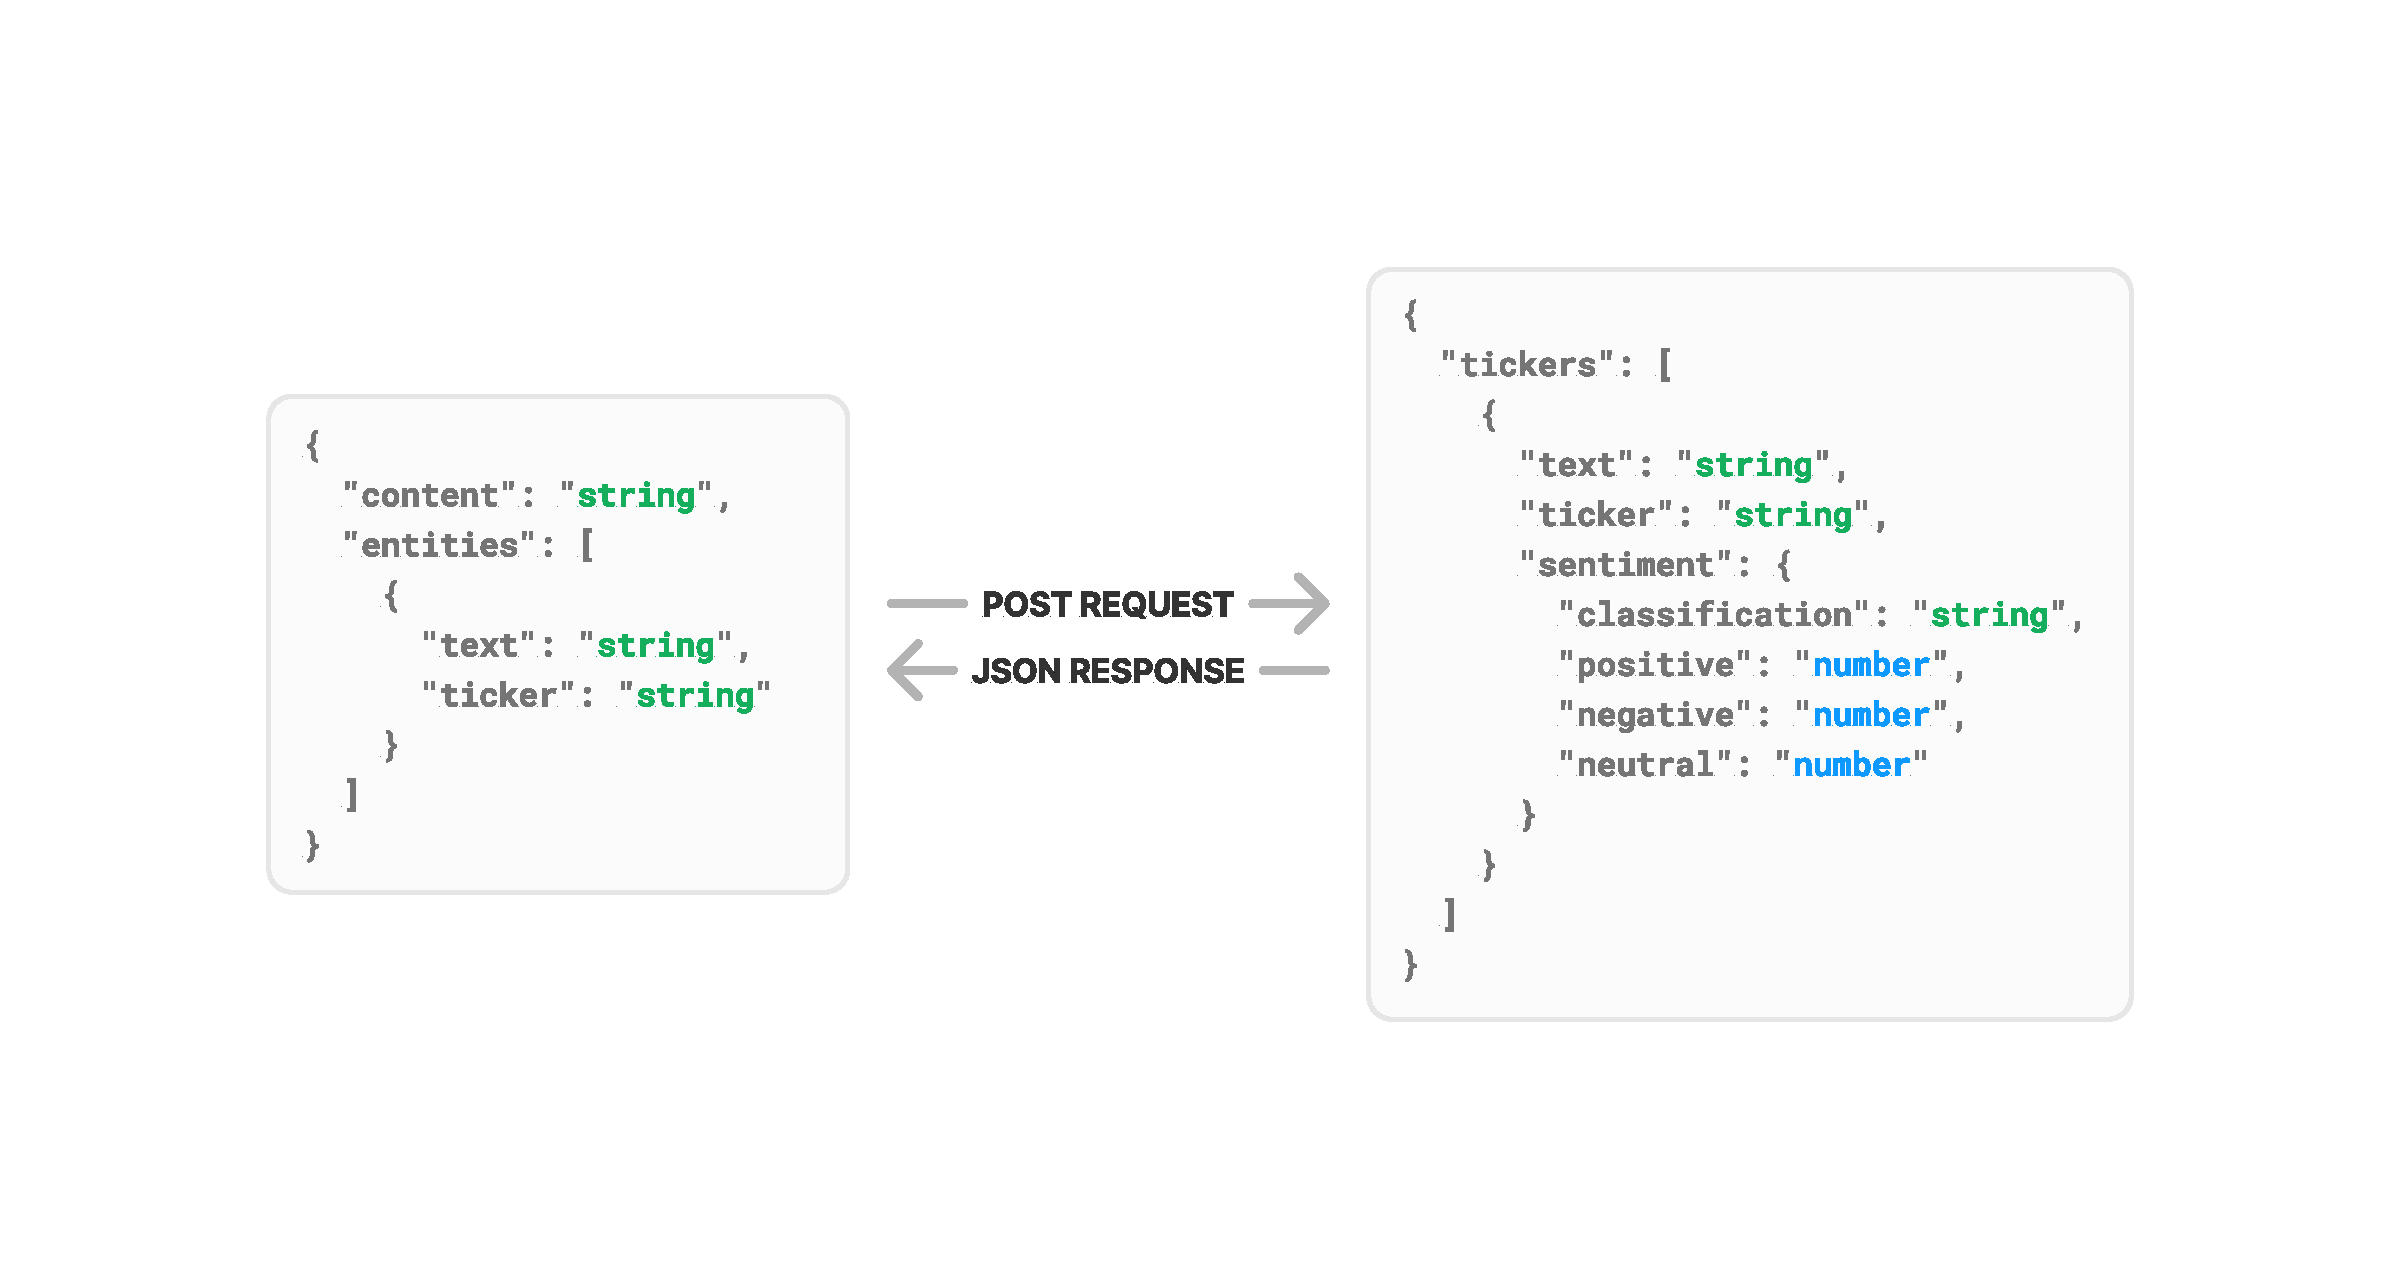
\includegraphics[width=\textwidth]{img/architecture/sa-req-res.pdf}
    \caption{Schema of a POST request to the SA service for sentiment analysis of extracted entities in article content and its reponse.}
    \label{fig:architecture-sa-req-res}
\end{figure}

Like the \acrshort{ner} service built on ASGI, the FastAPI framework was also selected for its speed and efficiency. Being built on ASGI enables FastAPI to be implemented asynchronously, which is beneficial for processing data from the \acrshort{ner} service. Despite sentiment analysis demanding more computational power, two workers also manage the endpoint. The interval we have set for repeating the \acrshort{dag} is $4$ hours, sufficient for processing speed, meaning processing takes $49$ minutes and repeats every $4$ hours.

\subsection{REST API Service}
\label{subsec:architecture-rest-api}
The \acrshort{restapi} service primarily provides access to data stored in the database. It is responsible for handling requests from the frontend and returning the appropriate data to be displayed to users. This service uses Flask\footnote{\href{https://www.flask.palletsprojects.com/en/3.0.x/}{https://www.flask.palletsprojects.com/en/3.0.x/}}, a lightweight Web Server Gateway Interface\footnote{\href{https://wsgi.readthedocs.io/en/}{https://wsgi.readthedocs.io/en/}} (WSGI) web application microframework. This framework is chosen for its flexibility, simplicity, and ease of extensibility. Most importantly, it provides more satisfactory control and management of schemas and resources than FastAPI, which is crucial for the purposes of this \acrshort{api}.

The \acrshort{api} handles the connection to the database using a controller, which grants access to all data from the \acrshort{etl} process. It scans whether temporary tables are available in the database during each request, which exists only during the \acrshort{etl} process. Furthermore, since the main tables are empty during \acrshort{etl}, it queries the replicated temporary tables. After the \acrshort{etl} process ends, these tables are removed, and the \acrshort{api} accesses the main tables containing data after the recent \acrshort{etl}. The \acrshort{api} is designed to handle frontend requests and provide responses with data in JSON format. Thus, the output is a JSON file containing data from the database, which is then displayed to users.

The \acrshort{api} provides the following endpoints, which we will not specify in detail with images like the previous two services but only summarise. We refer directly to the Swagger documentation, which we specify in more detail in Chapter \ref{chap:development-documentation}, for a detailed description of schemas and resources. Here is a summary of the endpoints, all of which are in the form of GET requests:

\begin{itemize}
    \item \textbf{Company Info} fetches a company's information from the database, as well as daily high and low prices and market volume from Yahoo Finance.
        \begin{itemize}
            \item \textit{/api/v0/company/\{ticker\}/info}
        \end{itemize}
    \item \textbf{Company Chart} fetches a company's chart data, such as sentiment, from the database and adjusted close price from Yahoo Finance to be displayed in chart.
        \begin{itemize}
            \item \textit{/api/v0/company/\{ticker\}/chart}
        \end{itemize}
    \item \textbf{Company Article List} fetches a company's articles from the database.
        \begin{itemize}
            \item \textit{/api/v0/company/\{ticker\}/articles}
        \end{itemize}
    \item \textbf{Company Graph} fetches a company's graph data from the database to be displayed as a graph network.
        \begin{itemize}
            \item \textit{/api/v0/company/\{ticker\}/graph}
        \end{itemize}
    \item \textbf{Companies Names and Tickers} fetches all companies' names and tickers from the database.
        \begin{itemize}
            \item \textit{/api/v0/companies/names}
        \end{itemize}
    \item \textbf{Companies Graphs} fetches all companies' graphs from the database to be displayed as a graph network.
        \begin{itemize}
            \item \textit{/api/v0/companies/graphs}
        \end{itemize}
\end{itemize}

\section{Frontend}
\label{sec:frontend}
The frontend is written using the Angular framework. Its principal function is to provide a user interface for interacting with data from the database through a \acrshort{restapi}. In our case, it communicates solely with the backend \acrshort{restapi} to retrieve and display data without making any updates. Built on top of TypeScript, Angular adds static typing and other features that simplify the development and implementation of the code. It offers many features, such as a modular architecture, which makes it easy to split an application into smaller parts, including components, services, and routing.

Although Angular is a frontend framework, infrastructure such as Docker or other server software is required to run it on a server. This infrastructure is used to deploy and serve the frontend application to users. Deploying an Angular application requires a server that provides users with static files. It is also built for single-page applications, which is an ideal solution in our case because the application can be more efficient, easily scalable, and maintainable, which is essential for long-term development. As part of the architecture and communication with other services, we create models in the form of interfaces that can be directly mapped to individual endpoints in the \acrshort{restapi}, which we can query its endpoints through an HTTP service.

The most significant benefit of Angular is its component architecture. The cornerstone is the component, composed of a TypeScript class, an HTML template, and styles typically in CSS. Components are reusable and can be easily moved to other application parts. This makes deploying new components smooth and effortless, increasing development efficiency. The flowchart navigation of application pages is illustrated in Figure \ref{fig:architecture-frontend-flowchart} below for a better understanding of the frontend structure. The following subsections describe each application component.

\begin{figure}[ht]
    \centering
    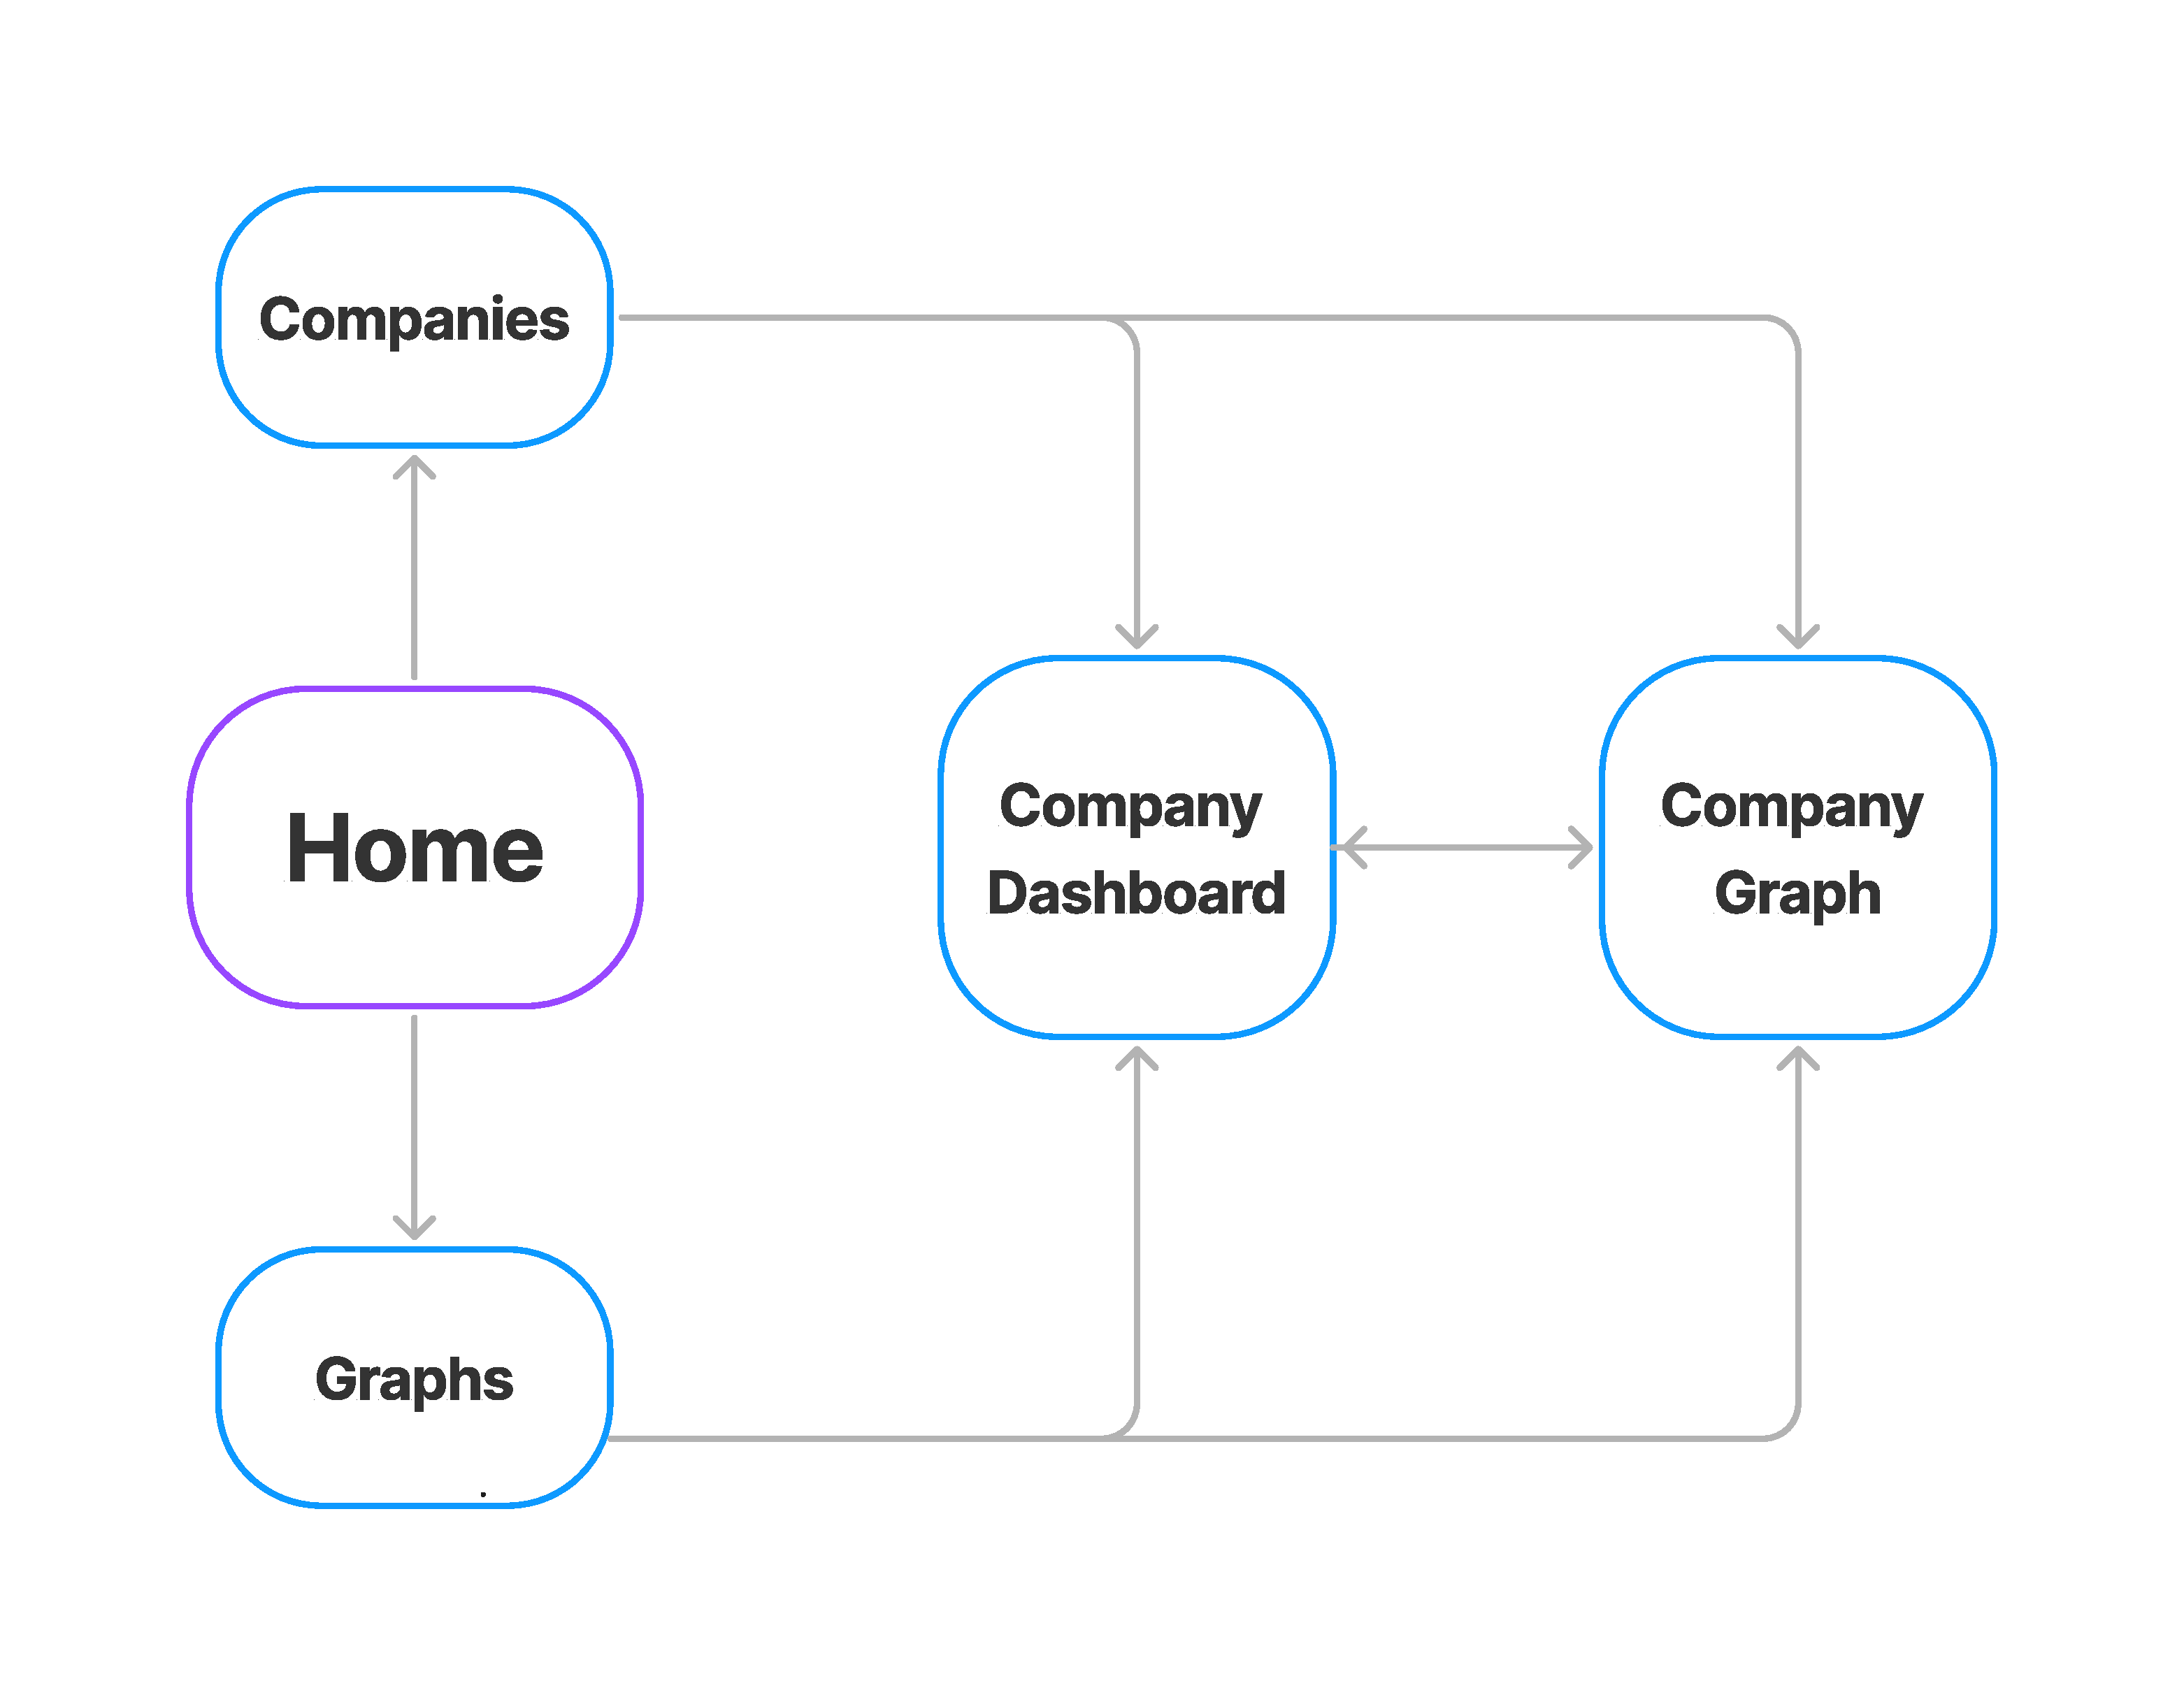
\includegraphics[width=0.7\textwidth]{img/architecture/website-flowchart.pdf}
    \caption{Flowchart navigation of application pages in the frontend.}
    \label{fig:architecture-frontend-flowchart}
\end{figure}

\subsection{Home Component}
\label{subsec:frontend-home}
This component serves as the homepage and does not contain any other components. It only displays an introduction describing the application. It includes a navigation bar, allowing users to access other application pages, such as graphs or companies.

\subsection{Graphs Component}
\label{subsec:frontend-graphs}
This component represents a page that displays the connections between individual articles and companies. The 3D Force Graph library, available on GitHub\footnote{\href{https://www.github.com/vasturiano/3d-force-graph}{https://www.github.com/vasturiano/3d-force-graph}}, provides the graph visualisation web component based on ThreeJS\footnote{\href{https://www.github.com/mrdoob/three.js/}{https://www.github.com/mrdoob/three.js/}}/WebGL for 3D rendering and d3-force-3d\footnote{\href{https://www.github.com/vasturiano/d3-force-3d}{https://www.github.com/vasturiano/d3-force-3d}} or ngraph\footnote{\href{https://www.github.com/anvaka/ngraph.forcelayout3d}{https://www.github.com/anvaka/ngraph.forcelayout3d}} for the core physics engine. An edge links an article to a company if the company is mentioned in the article. The edge colour represents the sentiment towards the company in the article. The colour of the articles varies based on their average sentiment towards all mentioned companies, while the company's colour is blue to distinguish it from the articles. Additionally, the edge colour indicates the sentiment associated with the specific company. 

The graph can be navigated and displayed, with control panels included for manipulating and modifying the graph visualisation. Users can filter the graph based on the average sentiment of individual articles and adjust the graph size to modify the visualisation. Each article can be viewed on the Guardian or navigated to the company graph or dashboard. The higher the mentioned companies within the article, the higher the article node size. The same applies to the company node. The higher mentioned in articles, the higher the company node size. We can smoothly identify the most trending companies in the articles. The interactive graph allows users to zoom in and out, rotate, and drag nodes. Additionally, graph traversal simulating the visibility of only neighbouring vertices is also implemented. The graph is loaded from the \acrshort{restapi} companies graphs endpoint.

\subsection{Companies Component}
\label{subsec:frontend-companies}
This component represents a page for searching individual companies' dashboards or graphs. It allows users to search for companies by name or ticker, implemented through Angular's ngx-pipes for efficient data manipulation and sorting by default. After searching, navigating to the selected company's dashboard or company graph component is possible. Like the home component, it also includes a navigation bar from which users can navigate to the graphs or home page. Data are loaded from the \acrshort{restapi} companies names and tickers enpoint.

\subsection{CompanyGraph Component}
\label{subsec:frontend-graph}
This component serves as a page, similar to the graphs component, but offers a slightly different view of the connections between individual articles and a specific company. The purpose is to reflect sentiment only to the individual company. Colouring in the graph works the same way as before. However, in this case, the article's node colours are based solely on the sentiment towards the specific company and not on the average sentiment of all the companies mentioned. Additionally, it contains control panels similar to those of the graph component. The graph is loaded from the \acrshort{restapi} company graph endpoint.

\subsection{CompanyDashboard Component}
\label{subsec:frontend-dashboard}
This component acts as a parent component to load individual child components. As the parent component, it loads data and then passes it to its children through the input decorator. This way, all data transfer is handled in one component, which then distributes it for loading. The child components of the company dashboard are as follows:

\begin{itemize}
    \item \textbf{CompanyInfo Component}: Displays brief information about the company.
    \item \textbf{Charts}: Individual charts are created using the CanvasJS\footnote{\href{https://www.canvasjs.com}{https://www.canvasjs.com}} library, which provides simple and efficient implementation within the Angular framework. Data for the charts is loaded from the \acrshort{restapi} company chart endpoint. The following charts are included:
    \begin{itemize}
        \item \textbf{StockChart Component}: Displays sentiment and adjusted close price in a stock chart average seniment for each day.
        \item \textbf{PieChart Component}: Shows the distribution of average sentiment over time in a pie chart.
        \item \textbf{SplineChart Component}: Illustrates each category of sentiment over time in a spline chart. 
    \end{itemize}
    \item \textbf{ArticleList Component}: Lists all articles mentioning the company, including relevant data such as title, date, link to the article, author, section, and sentiment. Data can be sorted and searched using text that applies to data in the table across all attributes. The listing is implemented through the material paginator provided by Angular. Data are loaded from the \acrshort{restapi} company article list endpoint.
\end{itemize}

By utilising the input decorator, data for all three charts is loaded only once, allowing us to clearly and efficiently create at least three charts without loading data separately for each chart. Additionally, data loaded into the CompanyInfo and ArticleList components come from specific endpoints explicitly created for their purpose. This approach allows us to effortlessly and efficiently implement additional components we want to include in the dashboard in the future.

Introduction
In today's era of information explosion and constant flow, it becomes more time-consuming to keep track of associations and deeply understand the published content through online news, primarily when investing in a specific area. The thesis aims to design and implement a tool to provide users with sentiment analysis of news articles to aid investment decision-making. 

Textual Data
First-party data providers are preferable to third-party providers because they offer higher data quality and reliability as direct sources. This approach ensures that the data accurately reflects reality and complies with terms of service, avoiding legal issues. First-party providers also have better specifications and defined APIs, making them more reliable.

Company to Symbol Linking
Three naive approaches on static datasets were presented to link company names to ticker symbols. They have limitations with name variations. A more efficient method is enhanced by a trained knowledge base on Wikidata, offering a structured data repository. Using the Spacy Entity Linker library in Python, we can match text entities to Wikidata entries and obtain additional entity information via SPARQL queries. This method covers most companies traded or related to those on exchanges, achieving nearly 100% success depending on the current entity's relationship with the exchange.

Entity-level Sentiment Analysis
The FinABSA model, trained on the SEntFiN 1.0 dataset, is ideal for this task. The model categorises sentiments into positive, neutral, and negative classes, providing numerical sentiment analysis. The FinEntity dataset, containing paragraphs from newspaper articles, entity annotations, and corresponding sentiments, is suitable for validating the algorithm. After significantly reducing the dataset to ensure precise measurement, the experiment achieved a 92% success rate with high accuracy. The correlation between entity-level sentiment and adjusted close prices of stocks demonstrates promising relationships, highlighting the potential of sentiment analysis in financial markets.

Implementation and architecture:
The application's high-level architecture contains individual services and their communication. The backend is divided into several services, each with a distinctly defined role. The ETL service is responsible for acquiring data from external sources, transforming it, and storing it in the database. The NER service categorises entities in article content data, while the SA service analyses the sentiment of text at the entity level. The REST API service provides access to data stored in the database. The frontend is written using the Angular framework, providing a user interface for interacting with data from the database through a REST API. The application's components include the Home, Graphs, Companies, CompanyGraph, and CompanyDashboard components.

The tool enables the particular analysis and provide a user-friendly and parameterisable visualisation of the results and their correlation with the stock market using a selected sentiment analysis approach. Each crucial architecture component is verified on a selected set of historical data. The architecture of the system is modular so that it ensures adding/replacing the analytical approaches, as well as integrating new types of input data.